\documentclass[a4paper, 10pt]{article}
\usepackage[utf8]{inputenc}
\usepackage{verbatim}
\usepackage{listings}
\usepackage{graphicx}
\usepackage{a4wide}
\usepackage{color}
\usepackage{amsmath}
\usepackage{amssymb}
\usepackage[dvips]{epsfig}
\usepackage[toc,page]{appendix}
\usepackage[T1]{fontenc}
\usepackage{cite} % [2,3,4] --> [2--4]
\usepackage{shadow}
\usepackage{hyperref}
\usepackage{titling}
\usepackage{marvosym }
\usepackage{physics}

\usepackage{subcaption}
\usepackage[noabbrev]{cleveref}
\usepackage{wasysym}
\usepackage{changepage}


\renewcommand{\topfraction}{.85}
\renewcommand{\bottomfraction}{.7}
\renewcommand{\textfraction}{.15}
\renewcommand{\floatpagefraction}{.66}
\renewcommand{\dbltopfraction}{.66}
\renewcommand{\dblfloatpagefraction}{.66}
\setcounter{topnumber}{9}
\setcounter{bottomnumber}{9}
\setcounter{totalnumber}{20}
\setcounter{dbltopnumber}{9}


\setlength{\droptitle}{-10em}   % This is your set screw

\setcounter{tocdepth}{2}

\lstset{language=c++}
\lstset{alsolanguage=[90]Fortran}
\lstset{basicstyle=\small}
\lstset{backgroundcolor=\color{white}}
\lstset{frame=single}
\lstset{stringstyle=\ttfamily}
\lstset{keywordstyle=\color{red}\bfseries}
\lstset{commentstyle=\itshape\color{blue}}
\lstset{showspaces=false}
\lstset{showstringspaces=false}
\lstset{showtabs=false}
\lstset{breaklines}
\title{FYS4411 - Project 2\\
	The restricted Boltzmannn machine applied to the quantum many body problem}
\author{Daniel Heinesen$^1$, Gunnar Lange$^2$ \& Aram Salihi$^2$\\
	\small $^1$Department of Theoretical Astrophysics, University of Oslo, N-0316 Oslo, Norway\\
	\small $^2$Department of Physics, University of Oslo, N-0316 Oslo, Norway}
\begin{document}
	\maketitle
	\begin{abstract}
	\begin{center}
	 NICE ABSTRACT! Also check out our \href{https://github.com/dulte/FYS4411/tree/master/Project2}{GitHub}\footnote{\url{https://github.com/dulte/FYS4411/tree/master/Project2}}
\end{center}
	\end{abstract}
	\newpage
	\tableofcontents
	\newpage
	\section{Introduction}
	The interest in applying machine learning methods to quantum mechanical system has experienced a veritable surge in recent years, and many different methods and applications are currently being explored (see e.g. \cite{Broecker2017} or \cite{Botu2015}). A particularly interesting application of machine-learning to the quantum many-body system is presented by \cite{Carleo602}. They interpret the quantum many-body wavefunction as a system of exponential complexity, where we are interested in extracting some features, such as the energy. When viewed from this perspective, machine learning algorithms and neural networks are a natural way to attack the problem, as these are methods designed for extracting features from highly complex systems. They present a method which they title neural-network quantum states, where they use restricted Boltzmann machines to represent the wavefunction.\\
	\linebreak
	We apply their method to a system of fermions in an isotropic harmonic oscillator trap with Coloumb repulsion. This system has the advantage of being well-studied, as both analytic (\cite{0305-4470-27-3-040}) and numeric (\cite{PhysRevB.84.115302}) results are available for selected system configurations. This enables us to benchmark our results, and compare the performance of neural-network quantum states to other algorithms.\\
	\linebreak
	We focus on the ground state of our system, and therefore only investigate the case of $1$ and $2$ electrons, in $1$, $2$ and $3$ dimensions. We use restricted Boltzmann machines to attain the form of our wavefunction, and the use Variational Monte Carlo (VMC) methods to establish an upper bound on the ground state energy. The weights and biases in our neural network are minimized using a stochastic gradient approach with a fixed learning rate. We compare three different sampling methods in our VMC calculations - Metropolis sampling, importance sampling and Gibbs sampling. For each of these methods, we investigate how our system behaves as we vary the parameters associated with the system. We also include an analysis of the errors involved, using the blocking method.
	\section{Theory}\label{sec:Theory}
	\subsection{The Hamiltonian}
	We consider a $D$-dimensional system of $P$ electrons confined in an isotropic harmonic oscillator trap. Working in natural units ($\hbar=c=e=m_e=1$), the Hamiltonian of such a system is given by:
	\begin{equation}\label{eq:Hamiltonian}
	H=\sum_{i=1}^P \left(-\frac{1}{2}\nabla_i^2 +\frac{1}{2}\omega^2 r_i^2\right)+\sum_{i=1}^P \sum_{j=1}^{i}\frac{1}{r_{ij}}
	\end{equation}
	Here $\omega$ is the frequency of the oscillator trap, $r_{i}$ is the $D$-dimensional position vector of electron $i$ and $1/r_{ij}$ is the distance between electron $i$ and $j$. The first term describes the interaction of the electrons with the potential, and we refer to it as the noninteracting part. The second term describes the Coloumb interaction between the electrons, and we refer to it as the interacting part.\\
	\linebreak
	We now wish to find the energy, $E$ of our system, by solving the time-independent Schrödinger equation:
	\begin{equation}\label{eq:time_depenedent_schrodinger}
	H\Psi = E\Psi
	\end{equation}
	Where $\Psi$ is the wavefunction of the system.
	\subsection{Analytic solution}
	We are chiefly interested in the ground-state energy of our system, as this is the state that the system will fall into if left unperturbed by e.g. thermal excitation. If we ignore the interacting part, then we have an analytic solution to the ground-state wavefunction for two electrons, which according to \cite{Griffiths2004} is given by:
	\begin{equation}
	\psi(r_1,...,r_P)=C\exp\left(-\frac{\omega}{2}\sum_{i=1}^P r_i^2\right)
	\end{equation}
	Where $C$ is a normalization constant. Furthermore, the ground-state energy (in natural units) of such a system is given by:
	\begin{equation}\label{eq:Ground-state-energy}
	\frac{E}{\omega}=P\frac{D}{2}
	\end{equation}
	Note, however, that all of the above expressions are only valid up to $P=2$, as we are dealing with spin-1/2 fermions, to which the Pauli exclusion principle applies. Therefore, we can only have two particles in the ground-state, and these particles must have opposite spin. More precisely, they must be in the singlet state (total spin $0$) in the noninteracting case, as discussed in appendix \ref{ap:Derivative_spin}. In what follows, we therefore restrict ourselves to $P\in \{1,2\}$.\\
	\linebreak
	We also have analytic results for some special cases in the interacting case. In particular, according to \cite{0305-4470-27-3-040} and \cite{PhysRevB.84.115302}, the energy is $3$ (in natural units) for 2 particles in the 2-dimensional case with $\omega=1$.
	\subsection{The variational principle}
	 In the general case, where analytic solutions are not available, it is desirable to use a numeric method to find the ground state energy, or at least an upper bound on the ground state energy. We achieve such an upper bound by invoking the variational principle, as formulated in \cite{Griffiths2004}, which states that:
	\begin{equation}\label{eq:Variational_Principle}
	E_0\leq \frac{\langle \Psi_T | H |\Psi_T \rangle}{\langle \Psi_T | \Psi_T \rangle}
	\end{equation} 
	Where $E_0$ is the ground-state energy and $\Psi_T$ is any (not necessarily normalized) trial wavefunction for our system. We therefore choose a class of trial wavefunctions, $\Psi_T$, and then compute $E'=\langle \Psi_T | H |\Psi_T\rangle$ by using a Monte Carlo approach. The variational method then guarantees that our approximation to the energy, $E'$ will be larger than the ground state energy $E_0$. We then adjust our trial wavefunction within our class of wavefunctions, to give the lowest possible energy, hoping to attain a decent estimate for the actual ground-state energy of our system. 
	\subsection{Neural-network quantum states and Restricted Boltzmann Machines}
	To actually determine our class of trial wavefunction, we follow the approach outlined by \cite{Carleo602}. They choose to interpret the problem of solving equation \ref{eq:time_depenedent_schrodinger} as a multi-dimensional minimization and feature extraction problem. As neural networks were designed to tackle exactly this class of problem, we choose to employ a neural network to find our trial wavefunction.\\
	\linebreak
	We follow the approach advocated by \cite{Carleo602} and choose a restricted Boltzmann machine (RBM) as the basis for our neural network. Restricted Boltzmann Machines (RBM) are described in great detail in the literature, see e.g. \cite{Hinton2010}. We therefore provide only a rough outline on how to apply them. We begin by setting up a vector of $M$ visible nodes, $\mathbf{X}$, which corresponds to the position states of our system (with one state per particle, $P$ and dimension, $D$, i.e. $M=PD$), and a vector of $N$ hidden nodes, $\mathbf{H}$ which correspond to some feature of our system that we wish to use to predict our wavefunction. Each of these nodes have a bias associated with them, which determine their relative importance. Additionally, there are also weights associated with connections between the hidden nodes and the visible nodes, but there are no connections between nodes in the same layer (hence \textit{restricted} Boltzmann machine). The RBM method then consists of modelling the probability distribution for our system, given some visible nodes $\mathbf{X}$ and some hidden nodes $\mathbf{H}$, by a Boltzmann distribution function of the form:
	\begin{equation}
	F_{rbm}(\mathbf{X}, \mathbf{H})=\frac{1}{Z}\exp \left(-\frac{1}{T_0}E(\mathbf{X},\mathbf{H})\right)
	\end{equation}
	Where $Z$ is a normalization constant and $T_0$ is some reference temperature (set to $1$ in what follows). The energy, $E(\boldsymbol{X}, \boldsymbol{H})$ relates the weights and biases to the probability distribution. In the standard RBM formulation, both $\boldsymbol{X}$ and $\boldsymbol{H}$ are binary variables. We choose the hidden nodes $\boldsymbol{H}$ to be binary, $h_i \in \{0,1\}$. The visible nodes, $\boldsymbol{X}$, however, represent the position of the electrons in our system, and must therefore be modelled as a continuous function. We therefore use an extension of standard RBM known as Gaussian-Bernoulli Deep Boltzmann Machine's (GDBM), as described by \cite{Wang2014}. They implement the energy as:
	\begin{equation}
	E(\mathbf{X}, \mathbf{H})=\sum_{i=1}^{M}\frac{\left(X_i-a_i\right)^2}{2\sigma^2}-\sum_{j=1}^N b_j H_j -\sum_{i=1}^{N}\sum_{j=1}^{M}\frac{X_iw_{ij}H_j}{\sigma^2}
	\end{equation}
	Where $a_i$ is the bias associated with the visible node $X_i$, $b_i$ is the bias associated with the hidden node $H_i$ and $w_{ij}$ is the weight associated with the coupling between $X_i$ and $H_j$. As discussed in \cite{Wang2014}, this makes the marginal distribution of the $h_i$ Bernoulli distribution, whereas the marginal distribution of $X_i$ form a normal distribution with variance $\sigma^2$.\\
	\linebreak
	As our wavefunction is a function of the position coordinates only, we choose to interpret the marginal distribution of the visible nodes as our wavefunction. This marginal distribution is given by:
	\begin{equation}
	F_{rbm}(\mathbf{X})=\sum_{h_i \in \mathbf{H}}F_{rbm}(\mathbf{X}, \mathbf{H})
	\end{equation}
	Which gives, after some algebra done in \cite{Hjorth-Jensen2018}, our class of trial wavefunctions as:
	\begin{equation}\label{eq:Wavefunction}
	\Psi_T(\mathbf{X})=F_{rbm}(\mathbf{X})=\frac{1}{Z}\exp \left(-\sum_{i=1}^M \frac{(X_i-a_i)^2}{2\sigma^2}\right)\prod_{j=1}^{N}\left(1+\exp\left(b_j+\sum_{i=1}^M \frac{X_iw_{ij}}{\sigma^2} \right)\right)
	\end{equation}
	This trial wavefunction, given biases and weights $a,b,w$, is then plugged into equation \ref{eq:Variational_Principle} to find an upper bound on the ground-state energy of our system. We seek to optimize this wavefunction with respect to $a,b$ and $w$.
	\textbf{TALK ABOUT IF THIS CAN BE EXACT FOR NONINTERACTING}
	\subsection{Variational Monte Carlo methods}
	Having established our trial wavefunction, it remains to use the variational principle to estimate the ground state energy. We use a Monte Carlo approach to estimate the inner product given in equation \ref{eq:Variational_Principle}. A more detailed description of this may be found in \cite{Hjorth-Jensen2015}, and we therefore only sketch a procedure. We begin by considering the probability distribution associated with our trial wavefunction, given by:
	\begin{equation}
	P(\mathbf{X})=\frac{|\Psi_T|^2}{\int d\mathbf{X}|\Psi_T|^2}
	\end{equation}
	Where the normalization integral is to be carried out over all particles and dimension (i.e. over $M$ variables). If we now define the local energy (by solving equation \ref{eq:time_depenedent_schrodinger} for $E$) as:
	\begin{equation}\label{eq:Local_energy}
	E_L(\mathbf{X})=\frac{1}{\Psi_T}H\Psi_T
	\end{equation}
	Then the expectation value of the Hamiltonian (which gives the energy) is given by:
	\begin{equation}\label{eq:energy_in_state_space}
	E_0 \leq E[H]=\int d\mathbf{X}P(\mathbf{X})E_L(\mathbf{X})\approx \frac{1}{K}\sum_{i=1}^{K}E_{L,i}
	\end{equation}
	Thus, we can get an approximation to the ground state energy by averaging the local energy for various system configurations. This method is, however, contingent upon our ability to efficiently compute the local energy and sample the position space.
	\subsection{The local energy}
	The local energy is defined in equation \ref{eq:Local_energy}, with the Hamiltonian given in equation \ref{eq:Hamiltonian}. Note that the most complicated part of this expression is the second derivative of the wavefunction. We derive an analytic expression for this is in appendix \ref{ap:local_energy}. The local energy is then given by:
	\begin{equation}
	\begin{split}
	\frac{1}{\Psi_T}H\Psi_T=-\frac{1}{2}\sum_{k=1}^M\left[\frac{a_k-X_k}{\sigma^2}+\sum_{j=1}^N \frac{w_{kj}}{\sigma^2 \left(1+ \exp \left(-b_j-\sum_{i=1}^{M} \frac{X_iw_{ij}}{\sigma^2}\right)\right)}\right]^2\\
	+\frac{M}{2\sigma^2}-\frac{1}{2}\sum_{k=1}^M\sum_{j=1}^N \frac{w_{kj}^2 \exp \left(-b_j-\sum_{i=1}^{M}\frac{X_iw_{ij}}{\sigma^2} \right)}{\sigma^4\left(1+ \exp \left(-b_j-\sum_{i=1}^{M} \frac{X_iw_{ij}}{\sigma^2}\right)\right)^2}+\frac{1}{2}\sum_{i=1}^M\omega^2 X_i^2+\sum_{i=1}^P \sum_{j=1}^i \frac{1}{r_{ij}}
	\end{split}
	\end{equation}
	\subsection{Sampling the position space}
	To make sense of equation \ref{eq:energy_in_state_space}, we must sample our position space, to get a good estimate for the local energy of the system. We employ three different sampling techniques.	
	\subsubsection{The Metropolis algorithm}
	The Metropolis algorithm is described in further detail in \cite{Hjorth-Jensen2015}. We begin by noting that the wavefunction gives the probability of finding the particle at a point in position space. We will therefore get the most reliable estimates for our local energy if we sample where the wavefunction (and thus the probability distribution) is large, and we avoid wasting CPU cycles. The Metropolis algorithm is one way to achieve this. This is achieved by proposing to move a single particle according to:
	\begin{equation}\label{eq:metropolis_algorithm_step_size}
	\boldsymbol{r}_{\mathrm{i,new}}=\boldsymbol{r}_{\mathrm{i}}+\boldsymbol{\xi}dx
	\end{equation}
	Where $\boldsymbol{r}_{\mathrm{i}}$ is the position of particle $i$, $dx$ is a chosen step size and $\boldsymbol{\xi}$ is a D-dimensional vector of random numbers, whose distribution we discuss in section \ref{sec:met_propose_new_position}. To find out whether we should sample local energy at this new position, we compute the ratio:
	\begin{equation}\label{eq:transition_probability}
	\Theta=\frac{P(\boldsymbol{X}_{\mathrm{new}})}{P(\boldsymbol{X})}=\frac{|\Psi(\boldsymbol{X}_{\mathrm{new}})|^2}{|\Psi(\boldsymbol{X})|^2}
	\end{equation}
	Where $\boldsymbol{X}_{\mathrm{new}}$ is the position of the particles after updating the position of particle $i$ according to \ref{eq:metropolis_algorithm_step_size}. Note that this ratio determines if the particle is more likely to be found at the position $\boldsymbol{X}_{\mathrm{new}}$ than at position $\boldsymbol{X}$. The move is only accepted if $\Theta \geq \theta$, where $\theta\in[0,1]$ is a uniformly distributed random variable. Thus, if the probability of finding the particle at $\mathbf{X}_{\mathrm{new}}$ is larger than the probability of finding the particle at $\mathbf{X}$, then we accept the move. If not, then the larger the energy difference the less probable it is that the move is accepted. As such, we should eventually end up moving fairly close to the most likely position, without getting stuck in it.
	\subsubsection{The Metropolis-Hasting alogrithm/importance sampling}
	We compare the Metropolis algorithm to an alternative, known as importance sampling. This is described in further detail in \cite{Hjorth-Jensen2015}. Note that the Metropolis sampling described in the previous section picks positions at random, and as such does not have a preference for proposing steps that move the system to a region of high probability density (given by $|\Psi|^2$). As such, some CPU cycles will be wasted on positions that have a very small probability of occurring. Importance sampling seeks to alleviate this problem by introducing a quantum force, which "pushes" the system in the direction of high probability. This changes the way a new step is proposed, as discussed in section \ref{sec:met_propose_new_position}. This force is, on particle $i$ given by:
	\begin{equation}
	F_i(\boldsymbol{X})=\frac{2}{\Psi_T}\nabla_i \Psi_T=2\nabla_i \log \Psi_T
	\end{equation}
	We compute this in appendix \ref{ap:local_energy} and show that this force is given by:
	\begin{equation}\label{eq:quantum_force}
	F_i(\boldsymbol{X})=2\sum_{k=1}^D \left(\frac{a_k-X_k}{\sigma^2}+\sum_{j=1}^N \frac{w_{kj}}{\sigma^2 \left(1+ \exp \left(-b_j-\sum_{i=1}^{M} \frac{X_iw_{ij}}{\sigma^2}\right)\right)}\right)
	\end{equation}
	The analysis in \cite{Hjorth-Jensen2015} shows that the correct way to include this in our algorithm is by multiplying the transition probability $w$ defined in equation \ref{eq:transition_probability} by a Green's function given by:
	\begin{equation}
	G(\mathbf{X}, \mathbf{X}')=\frac{1}{(4\mathcal{D}\Delta t)^{3/2}}\sum_{i=1}^M \exp \left(-\frac{(X_i-X_i'-\mathcal{D}\Delta t F_i(\mathbf{X}'))^2}{4\mathcal{D}\Delta t}\right)
	\end{equation}
	Where $\mathcal{D}$ is a diffusion parameter, which in our case equals $1/2$. The modified transition probability is given by:
	\begin{equation}
	w_{\mathrm{importance}}=\frac{|\Psi(\boldsymbol{X}_{\mathrm{new}})|^2}{|\Psi(\boldsymbol{X})|^2}\frac{G(\boldsymbol{X}, \boldsymbol{X}_{\mathrm{new}})}{G(\boldsymbol{X}_{new}, \boldsymbol{X})}
	\end{equation}
	This transition probability is implemented exactly as in the previous section. 
	\subsubsection{Gibbs Sampling}
	Gibbs sampling is an alternative to Metropolis/Metropolis-Hastings algorithm, which is described in greater detail in \cite{Wang2014}. Here we have a more direct connection between the probability distribution of the neural network and the wavefunction. In order to establish a direct physical connection to the probability distribution of the RBM, we now model our wavefunction as:
	\begin{equation}\label{eq:wavefunction_Gibbs}
	\Psi_{T, \mathrm{Gibbs}} =\sqrt{F_{rbm}(\boldsymbol{X})}
	\end{equation}
	Where $\Psi_T$ is given in equation \ref{eq:Wavefunction}. Note that, as the wavefunction is real-valued, this implies $|\Psi_{T, \mathrm{Gibbs}}(\boldsymbol{X})|^2 = F_{rbm}(\boldsymbol{X})$, i.e. the marginal distribution directly models the position probability distribution.\\
	\linebreak
	We are also interested in the conditional distribution of the hidden nodes. This gives, after a few lines of Algebra done in \cite{Hjorth-Jensen2018}:
	\begin{equation}\label{eq:Marginal_distribution_H}
	\begin{split}
	P(H_j=1|\boldsymbol{X})=\frac{1}{1+\exp\left(-b_j-\frac{1}{\sigma^2}\sum_{i=1}^M X_i w_{ij}\right)}\\
	P(H_j=0|\boldsymbol{X})=\frac{1}{1+\exp\left(b_j+\frac{1}{\sigma^2}\sum_{i=1}^M X_i w_{ij}\right)}
	\end{split}
	\end{equation}
	We now initialize the weights, biases and position $\boldsymbol{X}$, as discussed in section \ref{sec:Initialization}. We can then compute the marginal distributions for $\boldsymbol{X}$ given in equation \ref{eq:Marginal_distribution_H}. We then draw a uniform random number $\theta \in [0,1]$ for each $H_i$, and update $H_i$ according to equation \ref{eq:Marginal_distribution_H}. Then the positions are updated according to their conditional distribution, which is, as shown in \cite{Hjorth-Jensen2018} \textbf{WRITE MORE HERE}
	\begin{equation}
	X_i\sim \mathcal{N}\left(\sum_{j=1}^Nw_{ij}H_j, \sigma^2\right)
	\end{equation}
	We then compute the local energy using this $\boldsymbol{X}$. Note that we here cannot use equation \ref{eq:Local_energy}, as this is only valid for $\Psi_T = F_{rbm}(\boldsymbol{X})$. However, the new expression for local energy only differs by some numerical factors to the previous expression, as discussed in appendix \ref{ap:derivative_gibbs}. 
	\subsection{Optimizing our wavefunction in parameter space}
	For our neural network to be successful, we must be able to minimize the energy of our wavefunction. This is done by varying the parameters $a_i$, $b_i$ and $w_{ij}$, and computing the local energy. The variational method then guarantees that the lowest energy we find will be larger than the ground state energy. We employ a stochastic gradient method to find the minimum in our parameter space. Defining a vector of all parameters, $\boldsymbol{\theta}$, we iterate this vector according to:
	\begin{equation}\label{eq:Minimization_theory}
	\boldsymbol{\theta}^{i+1}=\boldsymbol{\theta}^i + \gamma \frac{\partial \overline{E}_L}{\partial \boldsymbol{\theta}^i}(\boldsymbol{\theta}^i)
	\end{equation}
	Where $\overline{E}_L$ is the energy computed by means of the variational Monte Carlo method (given by equation \ref{eq:energy_in_state_space}) and $\gamma$ is the step size, which we vary. The derivative is with respect to all parameters. It is shown in \cite{Heinsen2018} that the derivative of this expectation value of the energy is given by:
	\begin{equation}
	\frac{\partial \overline{E}_L}{\partial \boldsymbol{\theta}}(\boldsymbol{\theta})=2\left(\left\langle \frac{1}{\Psi_T}\frac{\partial \Psi_T}{\partial \boldsymbol{\theta}}\overline{E}_L(\boldsymbol{\theta})\right\rangle-\left\langle \frac{1}{\Psi_T}\frac{\partial \Psi_T}{\partial \boldsymbol{\theta}}\right\rangle\left\langle \overline{E}_L(\boldsymbol{\theta})\right\rangle\right)
	\end{equation}
	We must therefore compute the derivative of our trial wavefunction, given in equation \ref{eq:Wavefunction}, with respect to all of our variational parameters.
	This is done in detail in appendix \ref{ap:derivative_parameters} for Metropolis/importance sampling and in appendix \ref{ap:derivative_gibbs} for Gibbs sampling. We iterate this method until the absolute value of our gradient, $\frac{\partial \overline{E}_L}{\partial \boldsymbol{\theta}}$  is small enough \textbf{DANIEL ADD STUFF}.
	\section{Methods}\label{Method_section}
	\subsection{An overview of the structure of our program}
	Our entire program may be found on our \href{https://github.com/dulte/FYS4411/tree/master/Project2}{GitHub}\footnote{\url{https://github.com/dulte/FYS4411/tree/master/Project2}}. It is an extension of the program presented in \cite{Heinsen2018}. The program consists of $3$ main classes:
	\paragraph{\texttt{main.cpp}}
	The main class first reads in the parameter files. It then sets up the initial guess for the weights of the neural networks and runs the stochastic descent method. Finally, it runs the full simulation with the optimized weights.\\
	\paragraph{\texttt{simulation.cpp}}
	This class contains the minimization method itself, and also runs the main Monte Carlo loop.
	\paragraph{\texttt{system.cpp}}
	The system class contains all the functions for the wavefunction, the different sampling methods, and the acceptance checks. It also contains the function for computing the local energy and the derivatives of the wavefunction as a function of the various parameters.\\
	\linebreak
	In addition, we implement various auxiliary classes, that read in parameters, dump variables to file and do statistical analysis. These are described in greater detail on our repository.
	\subsection{Initializing our system}\label{sec:Initialization}
	\subsubsection{Initializing the position}
	To initialize our system, we must distribute our particles. How we distribute the particles, however, depends on the sampling method employed. When using the Metropolis algorithm or Gibbs sampling, we distribute our particles according to:
	\begin{equation}
	\boldsymbol{r}_i=\boldsymbol{\xi}
	\end{equation}
	Where $\boldsymbol{\xi}$ is a vector of $D$ number, normally distributed with $\xi \sim 0.5\mathcal{N}(0,1)$ as we find that this gives a good spread.\\
	\linebreak
	When using importance sampling, however, we must distribute our particles slightly differently, as discussed in \cite{Hjorth-Jensen2015}. In this case, the initial distribution of particles is given by:
	\begin{equation}
	\boldsymbol{r}_i=\boldsymbol{\xi'}\sqrt{dx}
	\end{equation}
	Where $\boldsymbol{\xi'}$ is a vector of $D$ number distributed as $\mathcal{N}(0,1)$ and $dx$ is a step size which we tune, as described further in section \ref{sec:met_tuning_parameters}.
	\subsubsection{Initializing the parameters}
	We wish to minimize our wavefunction as a function of the biases $a$, $b$ and  the weights $w$. This is done by iterating equation \ref{eq:Minimization_theory}. However, we require an initial guess for the vector of parameters, $\boldsymbol{\theta}^0$. We choose this initial guess to be uniformly distributed in $[0, 0.01]$.
	\subsubsection{Initializing the simulation}
	To initialize the simulation, we set the parameters in the parameter file found on our \href{https://github.com/dulte/FYS4411/tree/master/Project2}{GitHub}$^1$. This gives the option to set a number of parameters of the system. Specifically, the parameter file allows the following parameters to be set at runtime:
	\begin{itemize}
	\item The number of Monte Carlo cycles
	\item The number of particles, $P$
	\item The number of hidden nodes, $N$
	\item The number of dimensions, $D$
	\item The oscillator frequency $\omega$
	\item The spread in the visible nodes, $\sigma$
	\item The diffusion parameter $D$ (setting this to $0$ deactivates importance sampling)
	\item The step size, $dx$
	\item The learning rate, $\gamma$
	\item Whether or not the system is interacting
	\item Whether the energy should be computed numerically or analytically
	\item Whether or not to use Gibbs sampling
	\end{itemize}
	\subsection{Proposing a new position}\label{sec:met_propose_new_position}
	As discussed in section \ref{sec:Theory}, both the Metropolis algorithm and the Metropolis-Hasting algorithm rely on proposing a new position of the system. The general form for this updating was given in equation \ref{eq:metropolis_algorithm_step_size}. We now discuss how this is concretely implemented for the different sampling method.\\
	\linebreak
	For straightforward Metropolis sampling, there is no bias in selecting this position. We therefore simply define the new position by:
	\begin{equation}
	\boldsymbol{r}_{\mathrm{i,new}}=\boldsymbol{r}_i+\boldsymbol{\xi}dx
	\end{equation}
	Where $\boldsymbol{\xi}$ consists of $D$ numbers, uniformly distributed in $[-1,1]$ and $dx$ is a step size.\\
	\linebreak
	For importance sampling, we add a bias in selecting the new position. This bias is introduced by including the quantum force, presented in equation \ref{eq:quantum_force}. The details of how to implement this bias are presented in \cite{Hjorth-Jensen2015}. This gives that the new step should be selected according to:
	\begin{equation}
	\boldsymbol{r}_{\mathrm{i,new}}=\boldsymbol{r}_i+\boldsymbol{\xi'}\sqrt{dx}+\mathcal{D}\boldsymbol{F}_i dx
	\end{equation}
	Where $\boldsymbol{F}_i$ is the quantum force on particle $i$, $\mathcal{D}$ is the diffusion parameter (equal to $1/2$) and $\boldsymbol{\xi'}\sim \mathcal{N}(0,1)$. Note that $dx$ may in general not be the same as above, and we investigate which $dx$ gives the best values for each case separately, as discussed in section \ref{sec:met_tuning_parameters}.
	\subsection{Implementing the optimization of the biases and the weights}
	To find the best trial wavefunction, we run the optimization algorithm given in equation \ref{eq:Minimization_theory} until the absolute value of the gradient is less than some $\epsilon$, or we have surpassed $100$ iterations. We use $100$ times fewer Monte Carlo cycles to compute the local energy in the optimization loop than in the actual simulation used to determine the energy.
	\subsection{The errors in our energy}
	We wish to provide error bounds on the energies that we find. Note that the local energies constitute a highly correlated system, as the state of the system in the current Monte Carlo step differs only by the position of a single particle from the state in the previous Monte Carlo step. The variance of the energy is therefore not a good indicator of the error in our system. Instead, we use a technique known as blocking. This is described in further detail in \cite{Jonsson2018} and we follow the same procedure as outline in \cite{Heinsen2018}.\\
	\linebreak
	Blocking works by averaging successive observations of the local energy. Such a pairwise operation preserves the variance of the data, but reduces the covariance of the data. We keep doing this until the covariance is small enough, as described in detail in \cite{Jonsson2018}. To ensure that we can this as frequently as possible, we let our number of Monte Carlo cycles be a power of $2$. 
	\subsection{Tuning the parameters}\label{sec:met_tuning_parameters}
	We note that our results are contingent upon a number of parameters, in addition to the biases and weights that our minimization algorithm tunes. Specifically, we must choose the learning rate, $\gamma$, the step size $dx$, the number of hidden nodes $N$, the spread in the visible nodes, $\sigma$ and the number of Monte Carlo cycles.\\
	\linebreak
	We tune each of these parameters in turn, hoping to get close to a global optimum in parameter space without having to do a complete stochastic descent. Note that the step size $\gamma$ and the number of hidden nodes $N$ are intimately related, as $\gamma$ determines the rate of convergence whereas $N$ determines the dimensionality of the convergence problem. We therefore choose to tune these parameters simultaneously, as they strongly influence one another.
	\subsubsection{Tuning the step size, $\boldsymbol{dx}$}
	The step size $dx$ determines how well we are able to sample the position space, as it describes how far our proposed next position should be from the previous position. To find the best possible step size $dx$, we investigate the behavior of the energy for different $dx$, and look at the acceptance rate. For this analysis, we fix some values of $\sigma,\gamma$ and $N$ that give acceptable values. We then choose a $dx$ that gives a good estimate of the energy, whilst having neither an extremely high nor an extremely high acceptance rate.\\
	\linebreak
	We first do this for the simplest possibles system ($1$ particle in $1$ dimension), checking both the brute-force Metropolis sampling and importance sampling (note that Gibbs sampling does not use a $dx$). For brute-force sampling, we accept a lower acceptance rate than for importance sampling, as importance sampling should lead to a higher acceptance rate.\\
	\linebreak
	We also do the same analysis for $2$ particles in $2$ dimensions, including interaction, as we have analytic answers for this system available in \cite{0305-4470-27-3-040}.
	\subsubsection{Tuning the spread in the visible nodes, $\boldsymbol{\sigma}$}
	We vary $\sigma$, using the $dx$ found above and acceptable values of $\gamma$ and $N$ and look at what energy we are able to attain. We do this only with Gibbs sampling, as this is where $\sigma$ is most relevant. We then use this $\sigma$ in the other cases as well. We do this separately for the simplest system ($1$ dimension, $1$ particle) and for the interacting system ($2$ dimensions, $2$ particles and interaction). We then use this $\sigma$ in all subsequent runs. 
	\subsubsection{Tuning the learning rate, $\boldsymbol{\gamma}$ and the number of hidden nodes, $\boldsymbol{N}$}
	We choose to tune the learning rate $\gamma$ and number of hidden nodes $N$ simultaneously, as explained above. We choose the values for $dx$ and $\sigma$ found previously, and look at the absolute value of the gradient as a function of the iterations of the minimization iterations. ($1$ particle and $1$ dimension). We then choose the combination of parameters that gives the lowest gradient over multiple iterations. We again do this separately for Metropolis sampling, importance sampling and Gibbs sampling, and separately for the simplest system ($1$ particle $1$ dimension) and the interacting system ($2$ particles, $2$ dimensions with interaction).
	\subsubsection{Choosing the number of Monte Carlo steps}
	Note that the numbers of Monte Carlo steps required will depend on the method used to sample the space, as e.g. importance sampling will accept more steps and therefore require fewer cycles. As we are limited to $2$ particles, however, we can afford to use a fairly large number of Monte Carlo cycles. We therefore choose to use enough Monte Carlo steps to ensure convergence in the uncertainty in the energy, and use the same number of Monte Carlo cycles independent of the sampling method. 
	\subsection{Benchmarking our results}
	Having chosen the parameters of our system, we can now benchmark our results. We look at the ground state energy for $1$ and $2$ particles, in $1$,$2$ and $3$ dimensions, both with and without interaction. Note that we have analytic results for the noninteracting case, given by equation \ref{eq:Ground-state-energy}, and that we have analytic results in the interacting case with $2$ dimension.\\
	\linebreak
	Note, that the variational principle only guarantees that we attain an upper bound on the ground state energy. As such, we can only check that our result is larger than or equal to the analytic result.
 	\section{Results}
	\subsection{Tuning our neural network quantum state in the simplest system}
	We begin by tuning the parameters of our NQS in the simplest possible case ($1$ dimension with $1$ particle).
	 \subsubsection{Tuning $\boldsymbol{dx}$}
	 We show the energy and acceptance rate using brute-force Metropolis sampling for various step sizes in figure \ref{fig:results_benchmark_no_importance} below:
\begin{figure}[ht!]
\centering
 \begin{subfigure}[b]{0.8\textwidth}
 	\centering
 	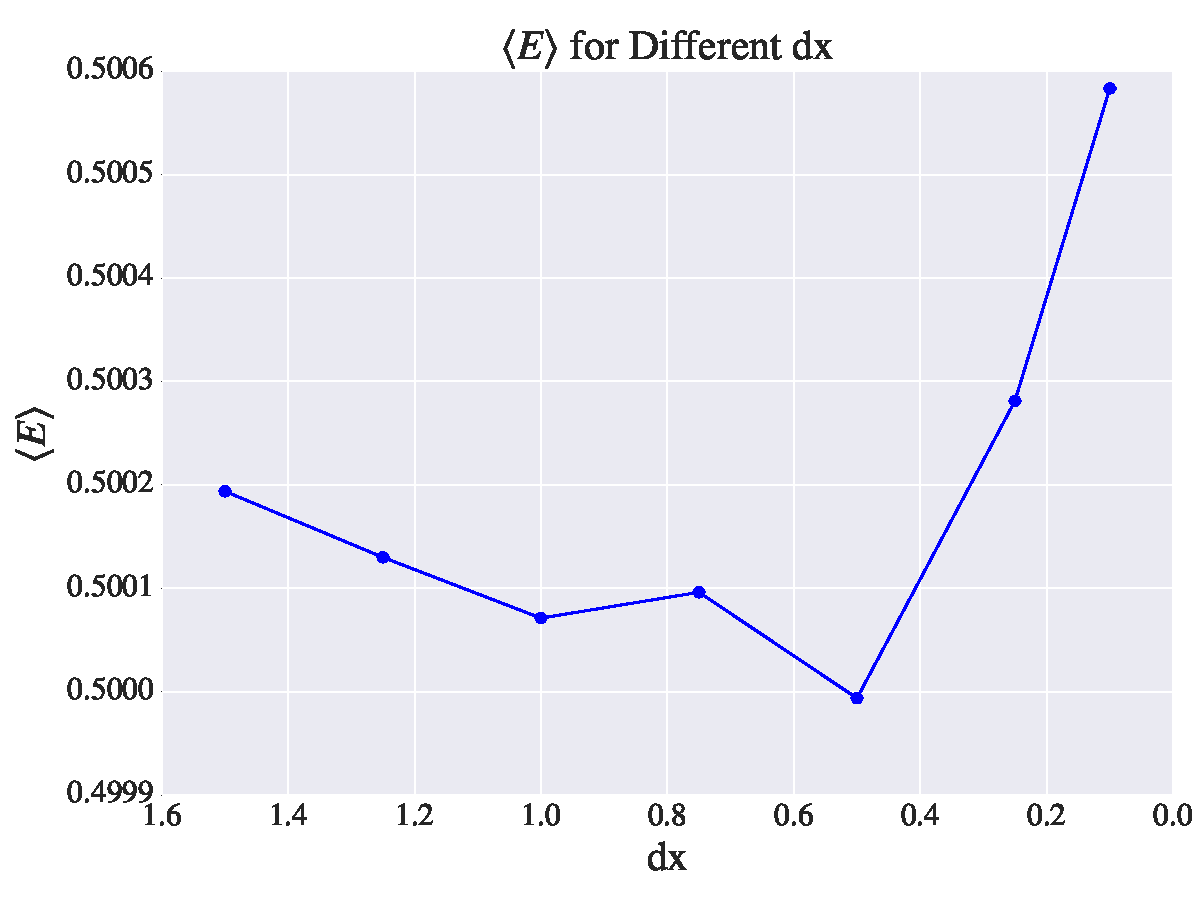
\includegraphics[width=\textwidth]{../Results/E_v_dx_normal.pdf}
 	\caption{Mean energy}
 \end{subfigure}
 ~
 \begin{subfigure}[b]{0.8\textwidth}
 	 	\centering
 	 	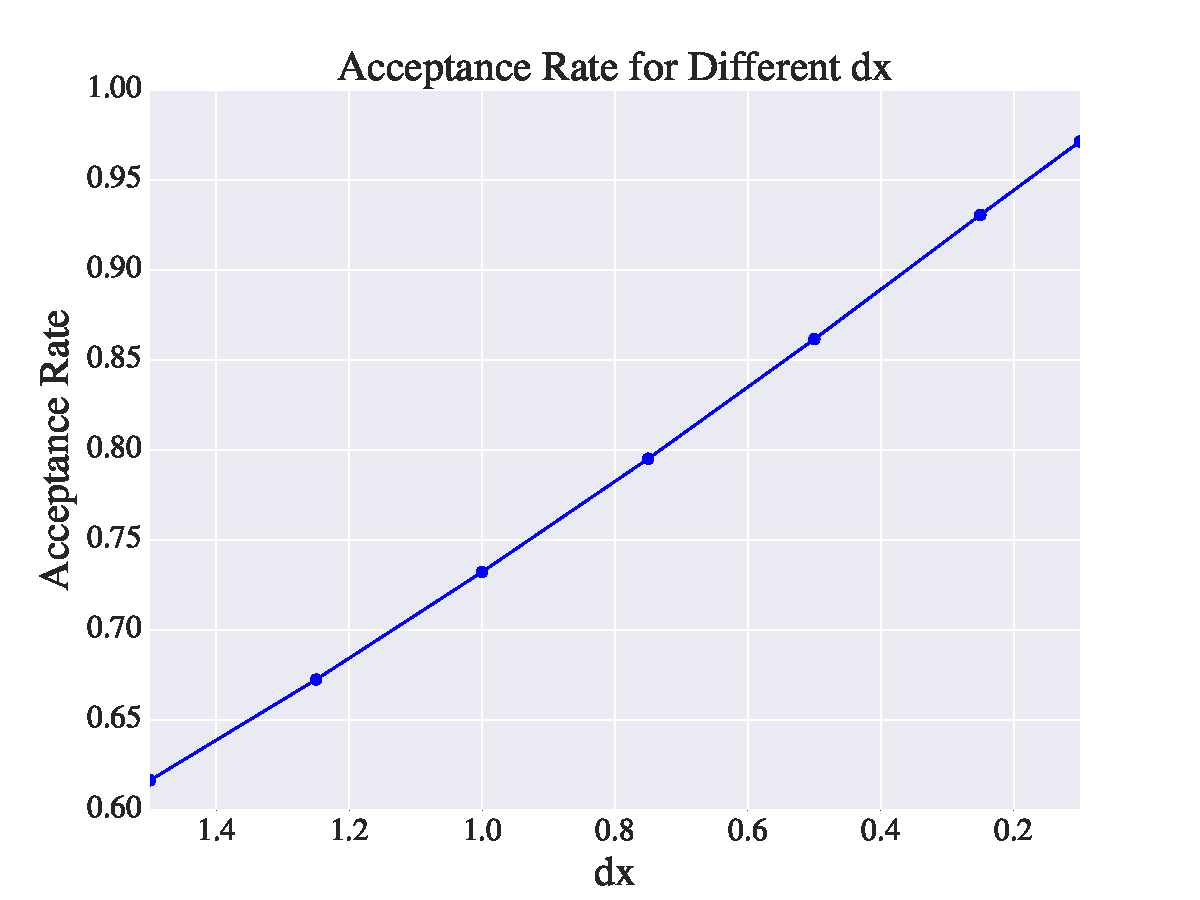
\includegraphics[width=\textwidth]{../Results/AC_normal.pdf}
 	 	\caption{Acceptance rate}
\end{subfigure}
\caption{Plot of the mean energy and corresponding acceptance rate for various values of $dx$, using $1$ particle in $1$ dimension and $2^{20}$ Monte Carlo steps \textbf{CHECK THIS}. This was produced using brute-force Metropolis sampling with $N=2$, $\gamma=0.3$ and $\sigma=1$.}\label{fig:results_benchmark_no_importance}
\end{figure}
As explained in section \textbf{SECTION}, we end up choosing $dx=1$. We show the equivalent plot with importance sampling in figure \ref{fig:results_benchmark_importance}
\begin{figure}[ht!]
	\centering
	\begin{subfigure}[b]{0.8\textwidth}
		\centering
		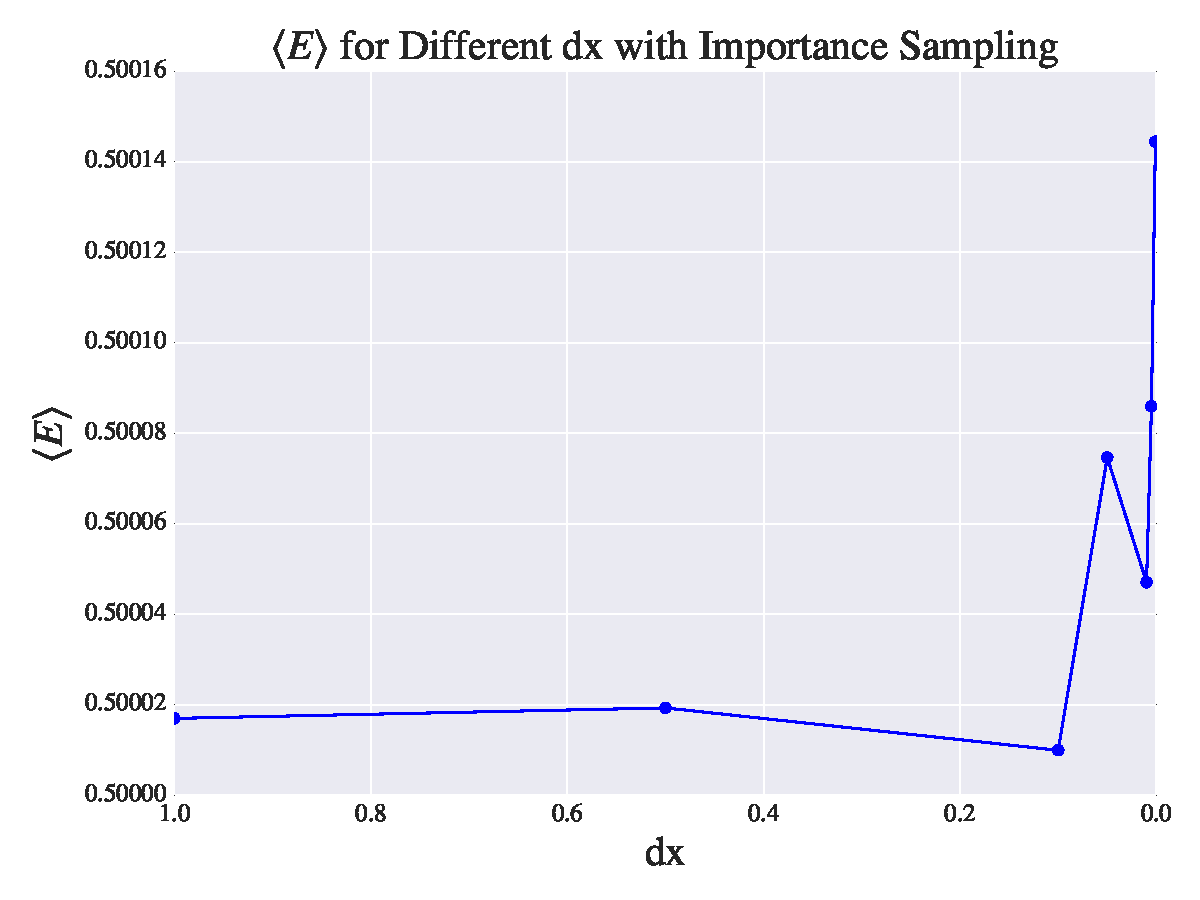
\includegraphics[width=\textwidth]{../Results/E_v_dx_importance.pdf}
		\caption{Mean energy}
	\end{subfigure}
	~
	\begin{subfigure}[b]{0.8\textwidth}
		\centering
		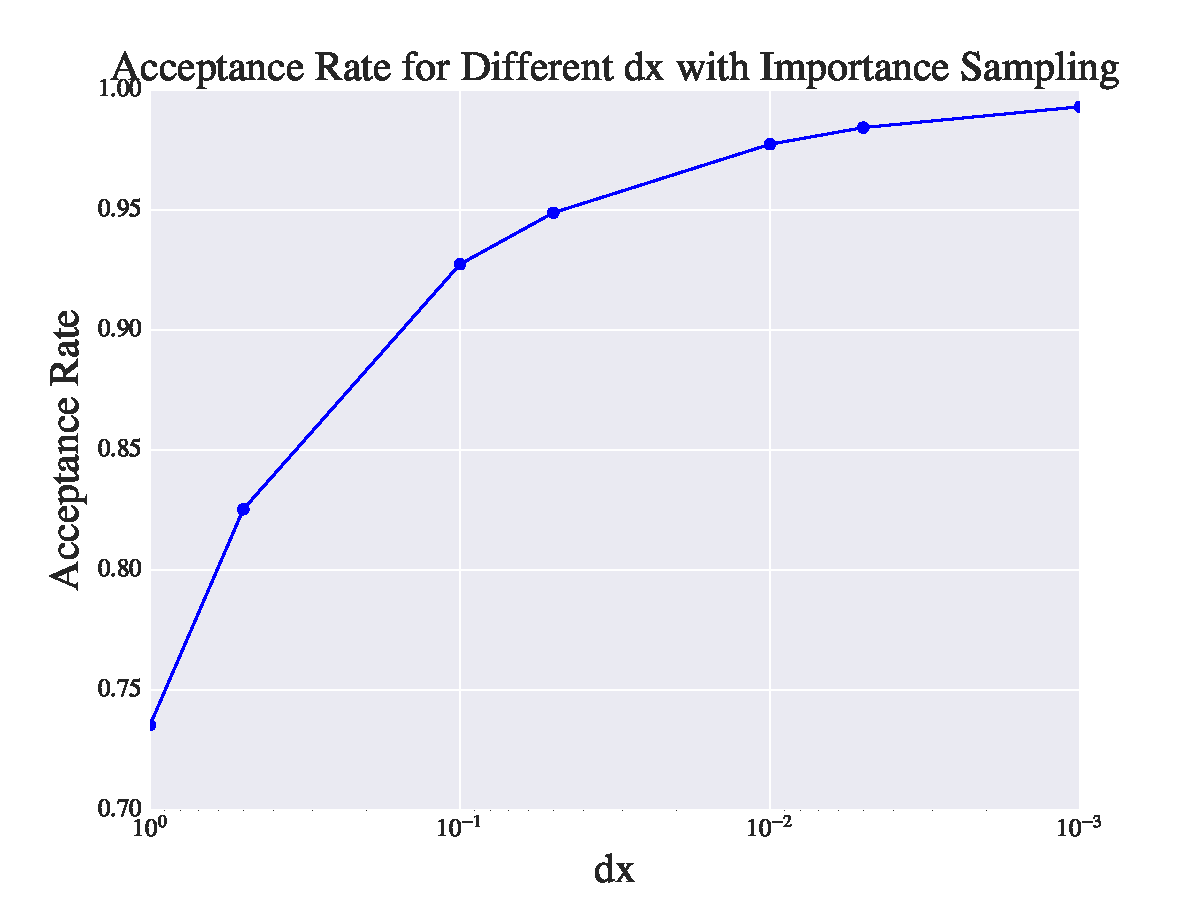
\includegraphics[width=\textwidth]{../Results/AC_importance.pdf}
		\caption{Acceptance rate}
	\end{subfigure}
	\caption{Same as figure \ref{fig:results_benchmark_no_importance}, but using importance sampling}\label{fig:results_benchmark_importance}
\end{figure}
In the case of importance sampling, we choose $dx=0.1$ as explained in \textbf{SECTION}.
\subsubsection{Tuning $\boldsymbol{\sigma}$}
We vary $\sigma$, using Gibbs sampling. This is shown in figure \ref{fig:sigma_1d}.
\begin{figure}
	\centering
	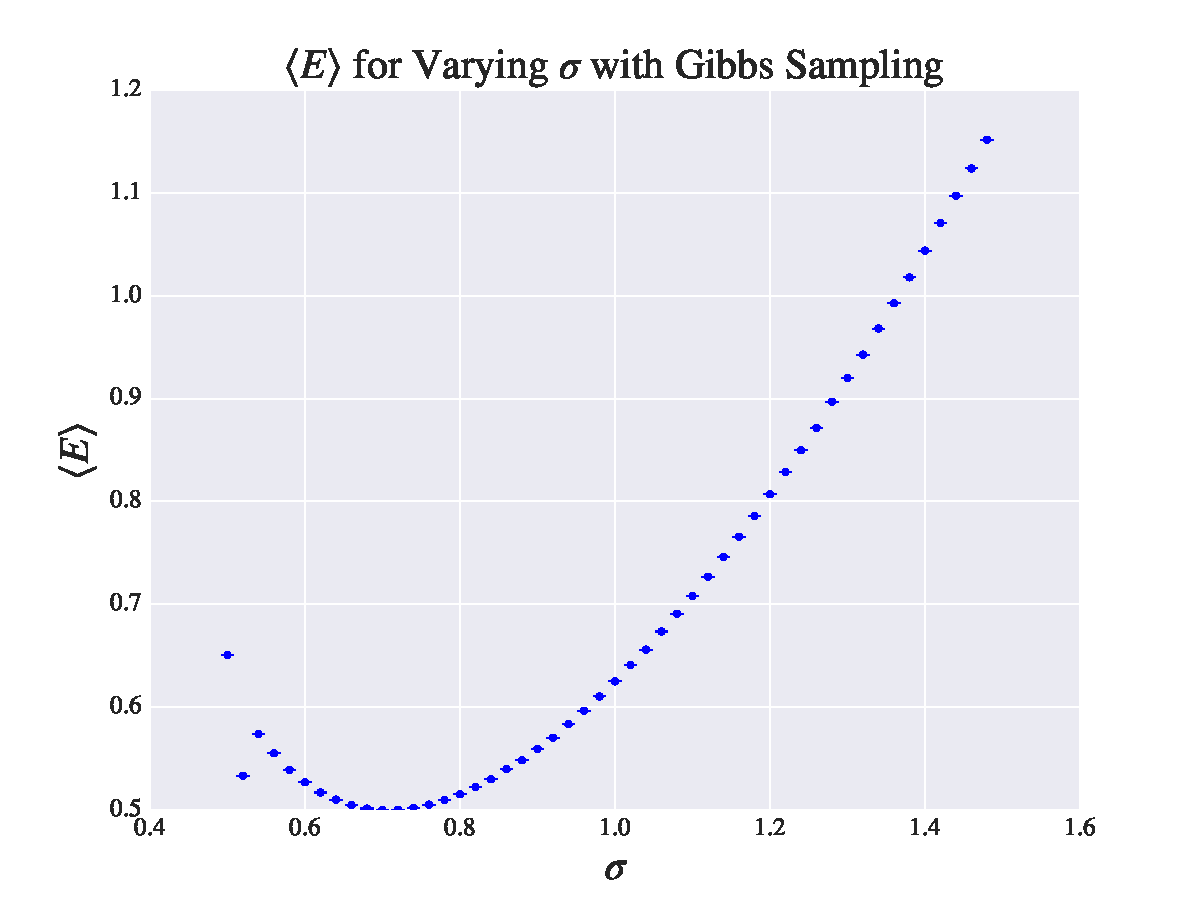
\includegraphics[width=\textwidth]{../Results/varying_sigma_gibbs.pdf}
	\caption{Mean energy for various values of $\sigma$ for a system of $1$ particle in $1$ dimension, using Gibbs sampling and $2^{10}$ Monte Carlo steps. This is with $N=2$ and $\gamma=0.3$}\label{fig:sigma_1d}
\end{figure}
As explained in section \textbf{SECTION}, we choose $\sigma=0.7$ in this case.
\subsubsection{Tuning $\boldsymbol{N}$ and $\boldsymbol{\gamma}$}
As discussed in section \textbf{SECTION}, we tune the learning rate, $\gamma$ and the number of hidden nodes, $N$ together. This gives the plot shown in figure \ref{fig:step_size_and_N_standard} for the standard Metropolis algorithm.
\begin{figure}
\centering
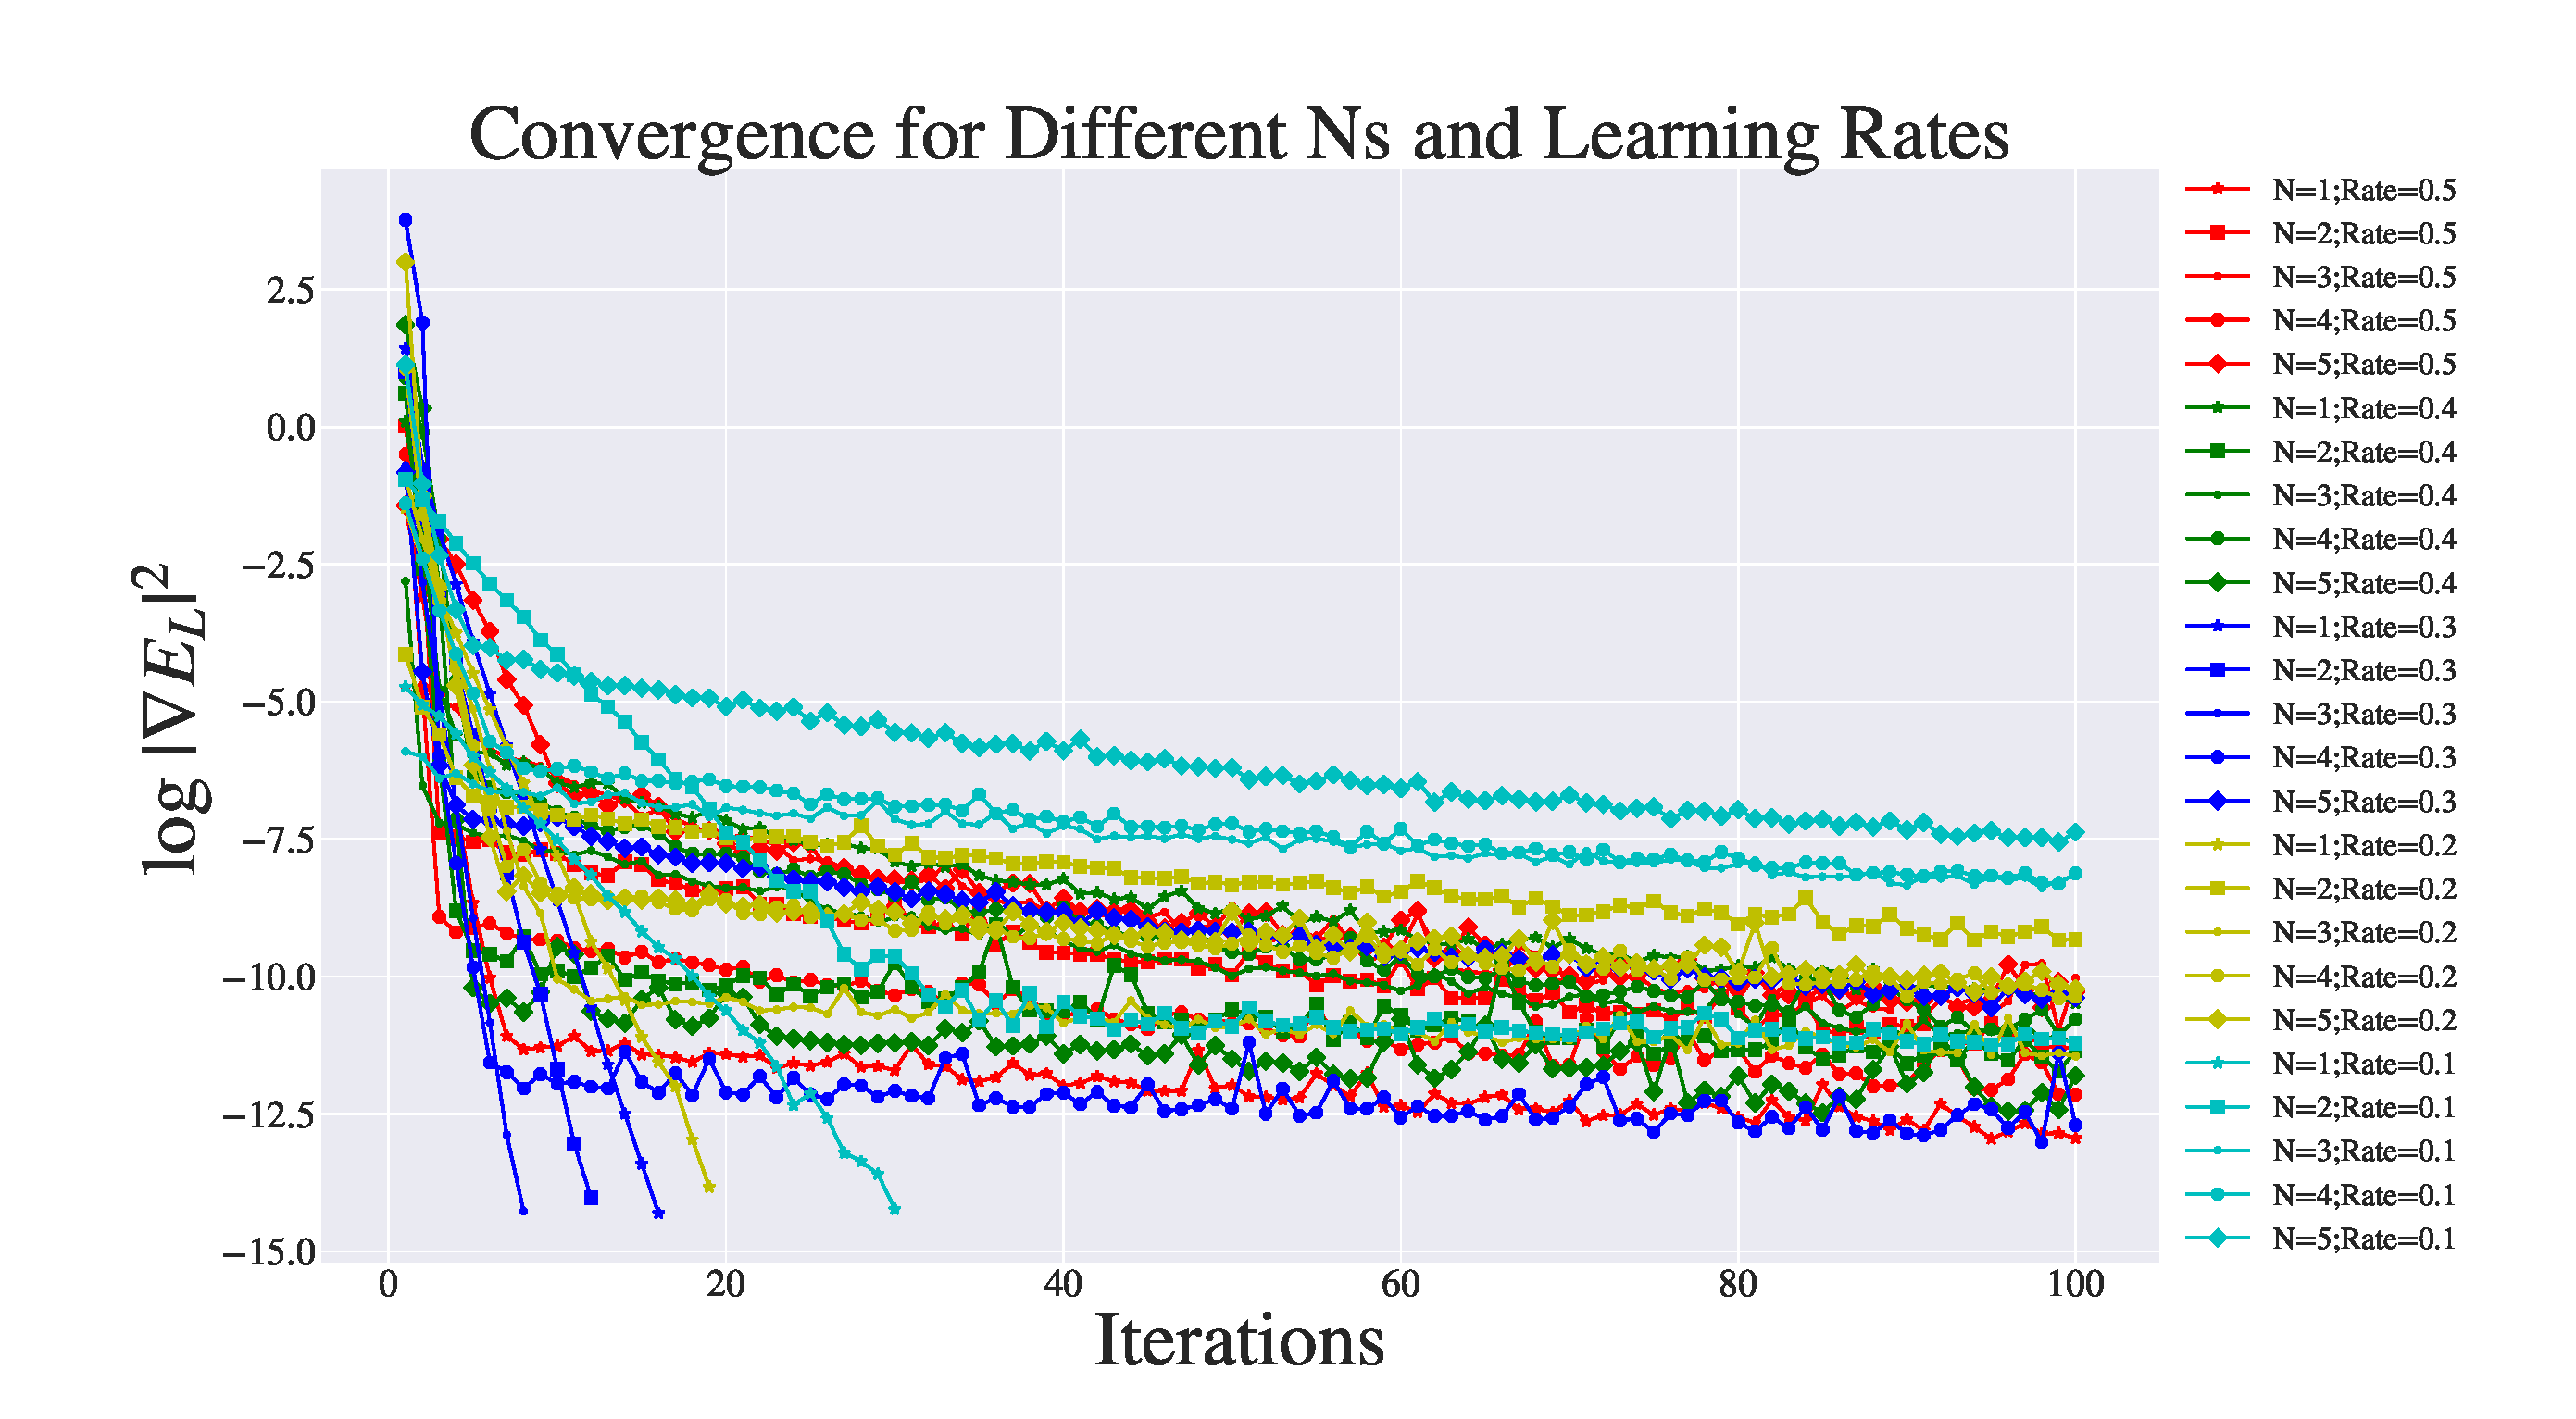
\includegraphics[width=\textwidth]{../Results/grad_normal.pdf}
\caption{Plot of the absolute value of the gradient as a function of iterations for various values of $N$ and $\gamma$. This was performed using brute-force Metropolis sampling, using $1$ particle in $1$ dimension and $2^{20}$ Monte Carlo cycles. We used $dx=1$, $\sigma=0.7$.}\label{fig:step_size_and_N_standard}
\end{figure}
As explained in section \textbf{SECTION}, we here choose \textbf{FINISH}.
The equivalent plot for importance sampling is shown in figure \ref{fig:step_size_and_N_importance}
\begin{figure}
	\centering
	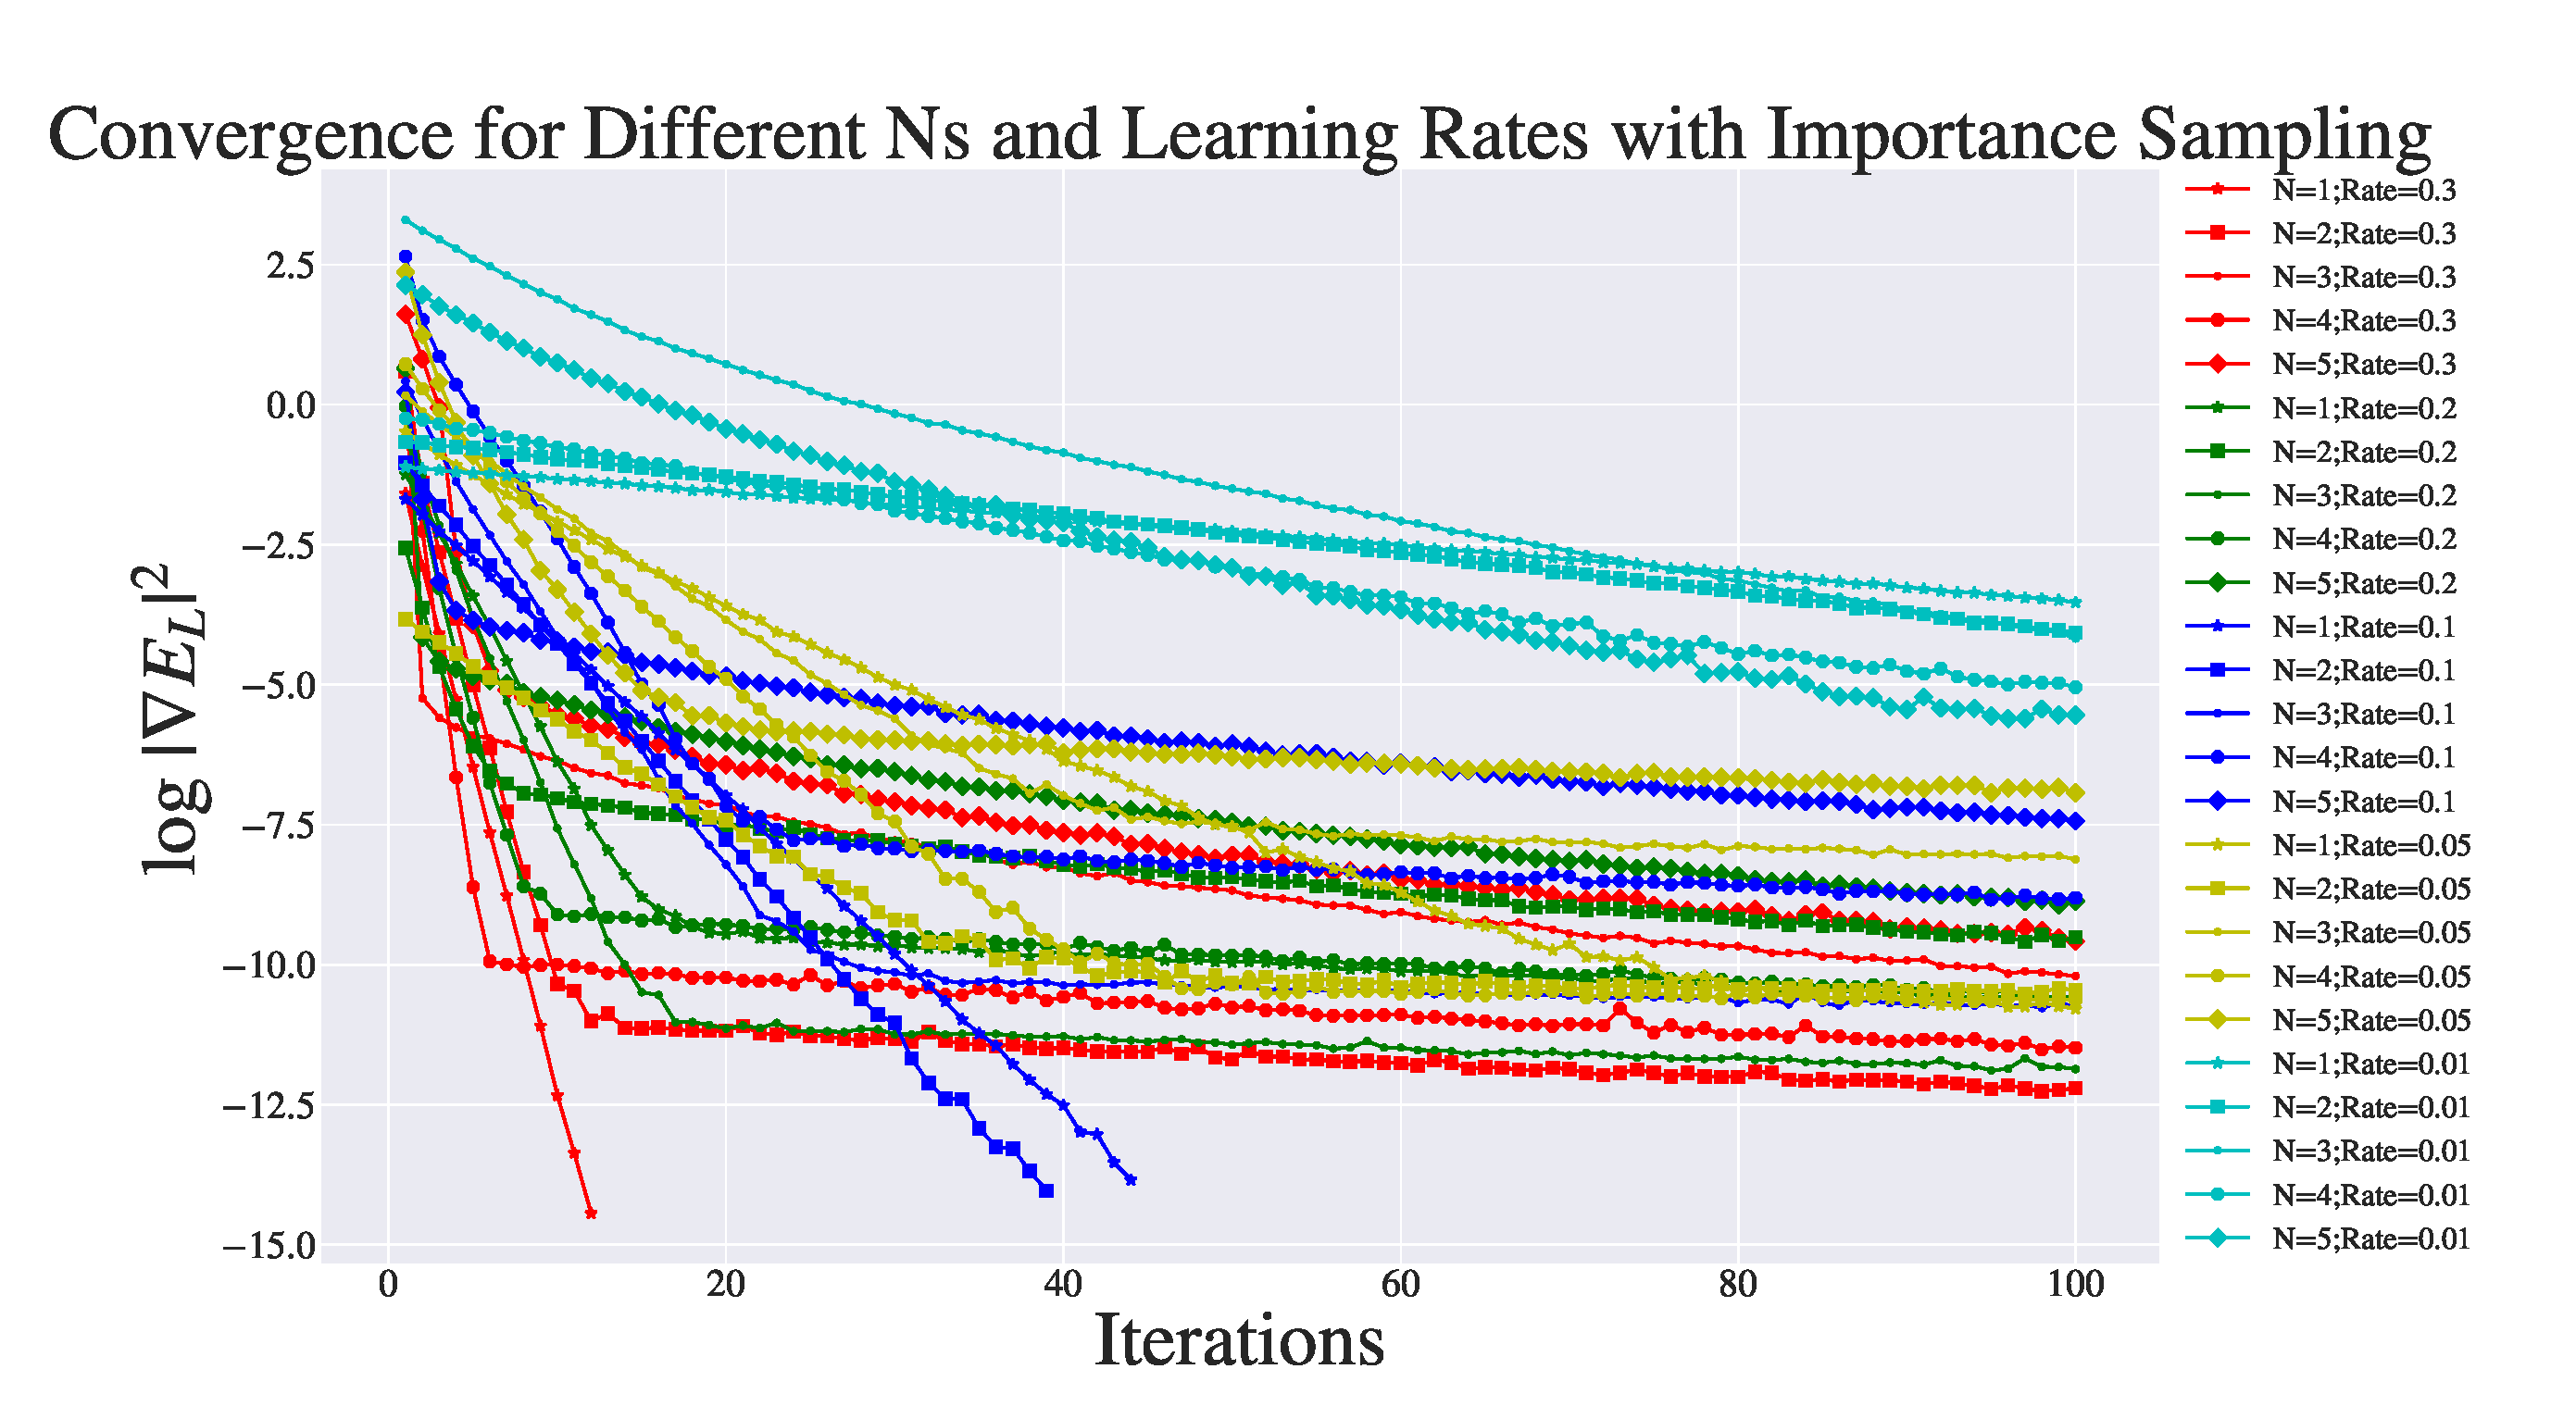
\includegraphics[width=\textwidth]{../Results/grad_importance.pdf}
	\caption{Same as figure \ref{fig:step_size_and_N_standard}, but using importance sampling, and therefore $dx=0.1$}\label{fig:step_size_and_N_importance}
\end{figure}
Here, we chose \textbf{FINISH}.
Finally, the same plot for Gibbs sampling is shown in figure \ref{fig:step_size_and_N_gibbs}
\begin{figure}
	\centering
	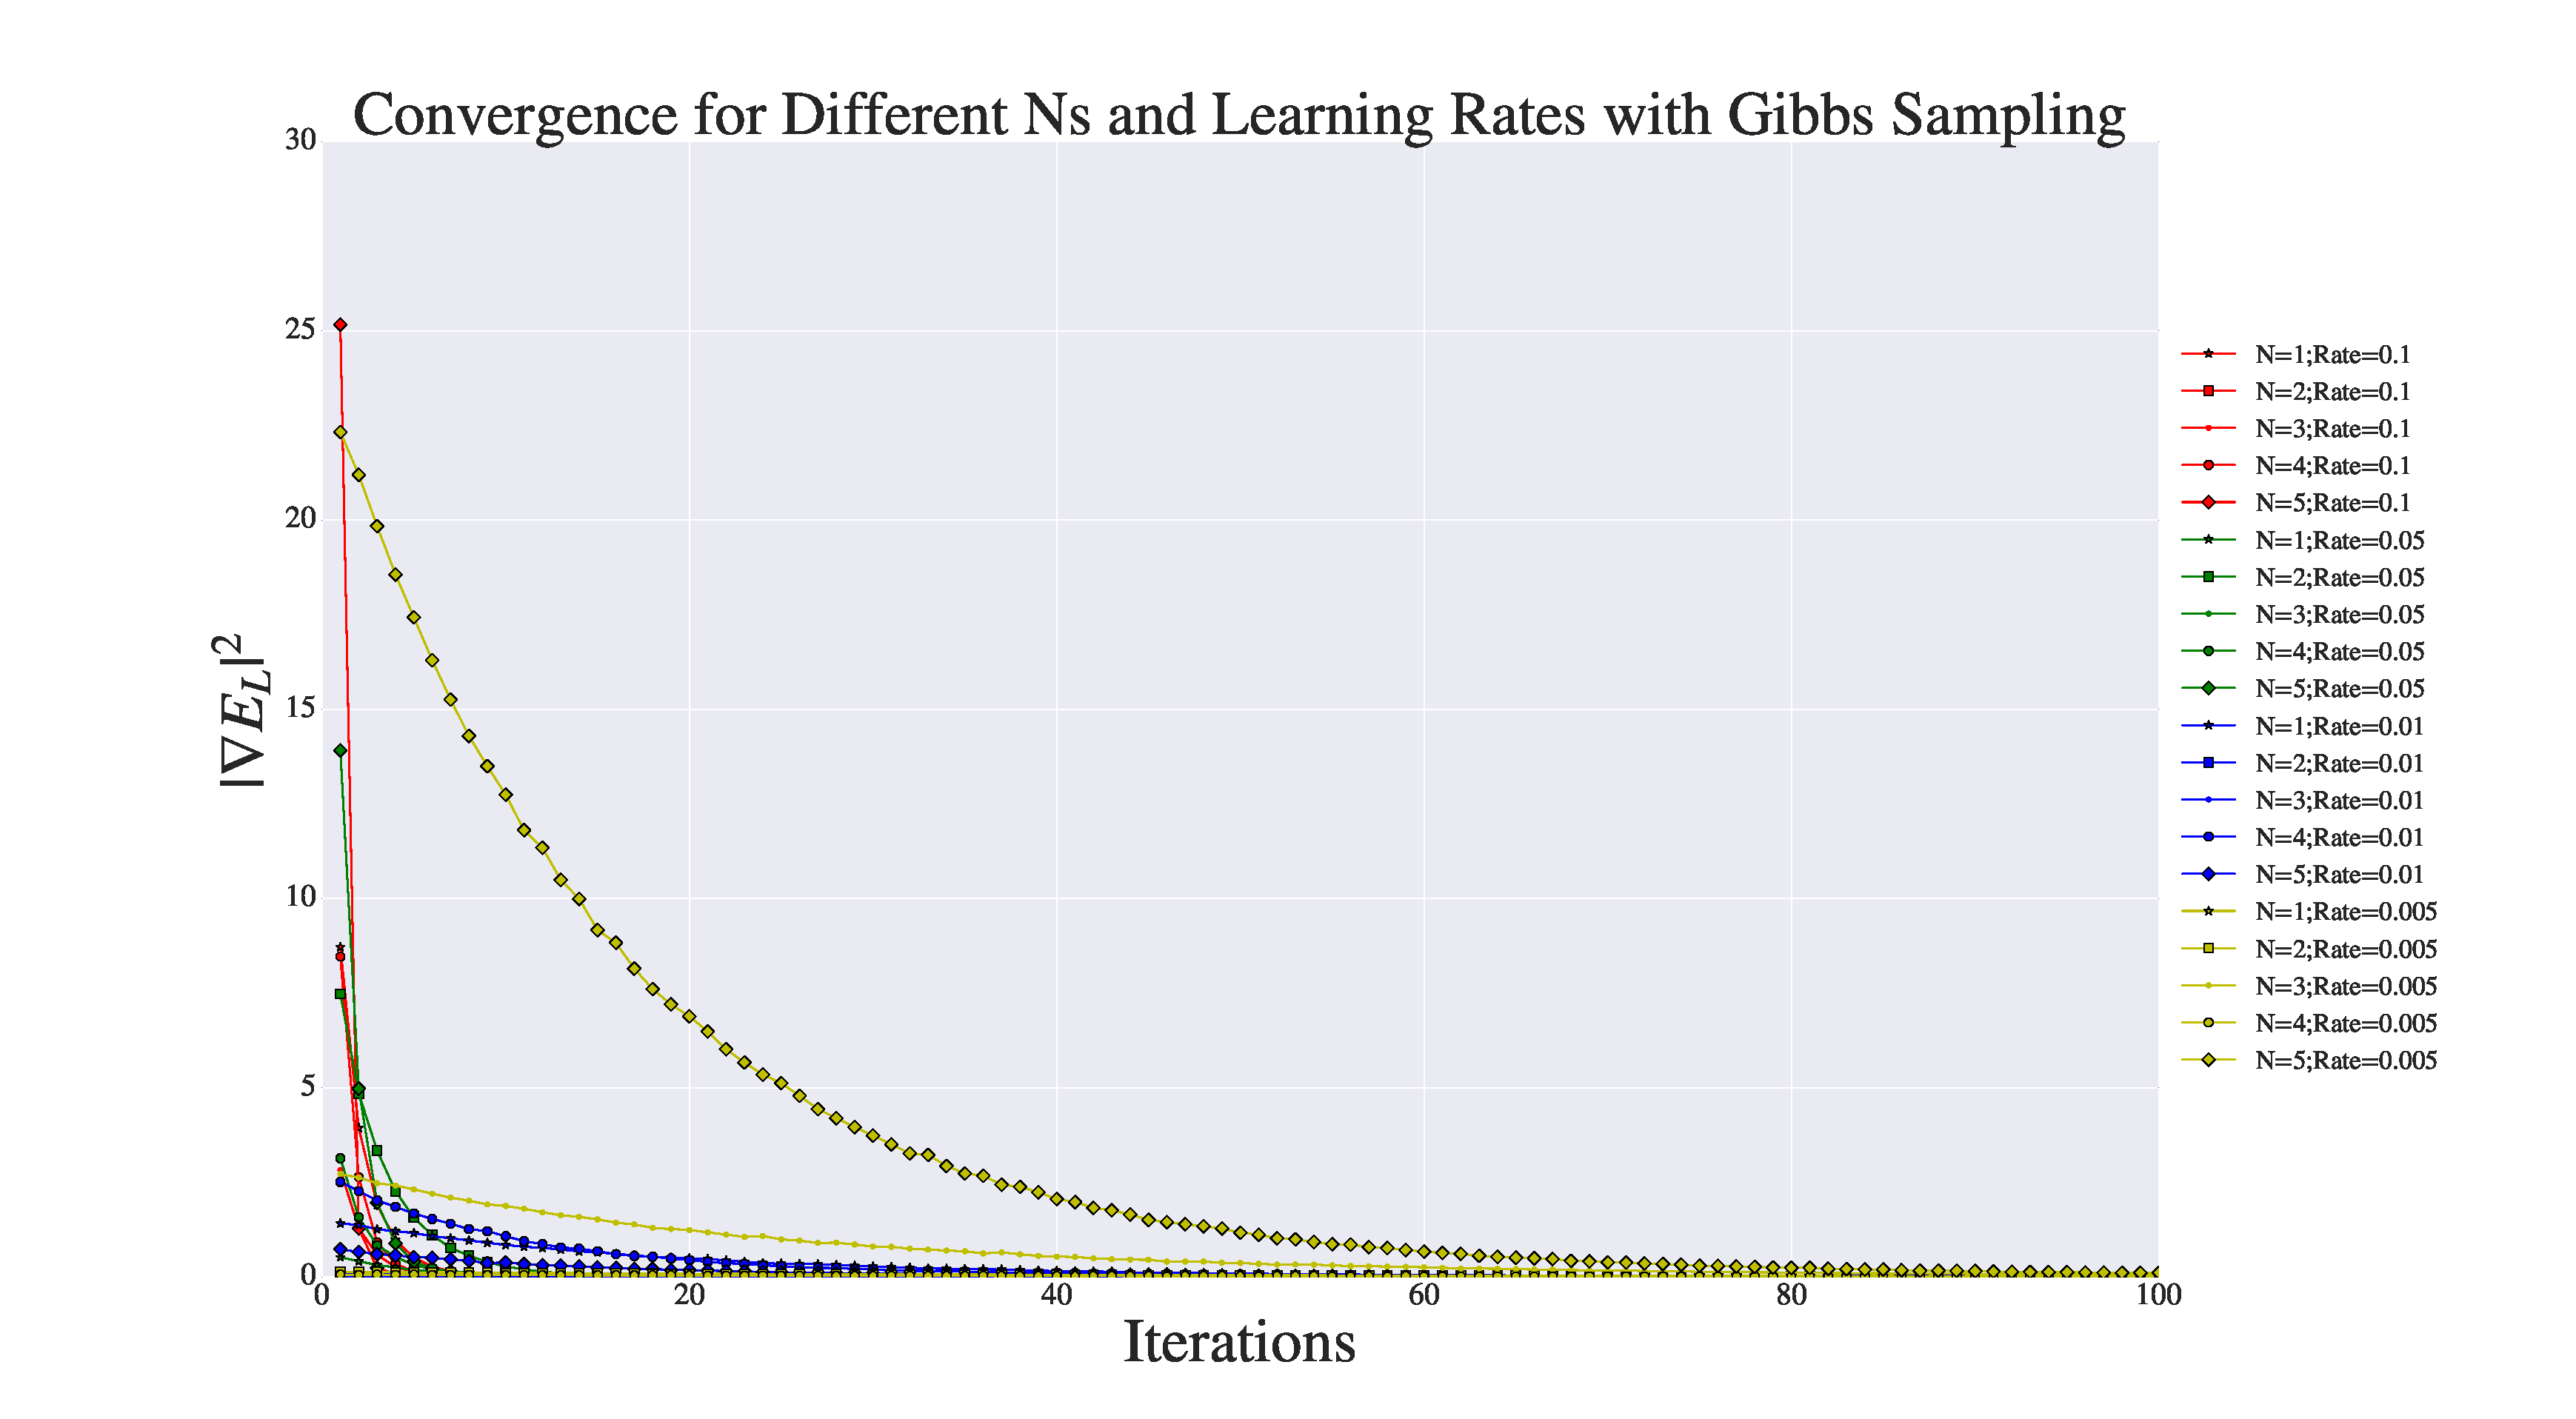
\includegraphics[width=\textwidth]{../Results/grad_gibbs.pdf}
	\caption{Same as figure \ref{fig:step_size_and_N_standard} but using Gibbs sampling}\label{fig:step_size_and_N_gibbs}
\end{figure}
\subsection{Tuning our neural network quantum state in the interacting system}
We perform the same analysis as in the previous section also in the interacting system with $2$ particles in $2$ dimension. 
	 \subsubsection{Tuning $\boldsymbol{dx}$}
	 We show the results of tuning the step size in the interacting case in figure \ref{fig:results_benchmark_no_importance_interacting} below:
	 \begin{figure}[ht!]
	 	\centering
	 	\begin{subfigure}[b]{0.8\textwidth}
	 		\centering
	 		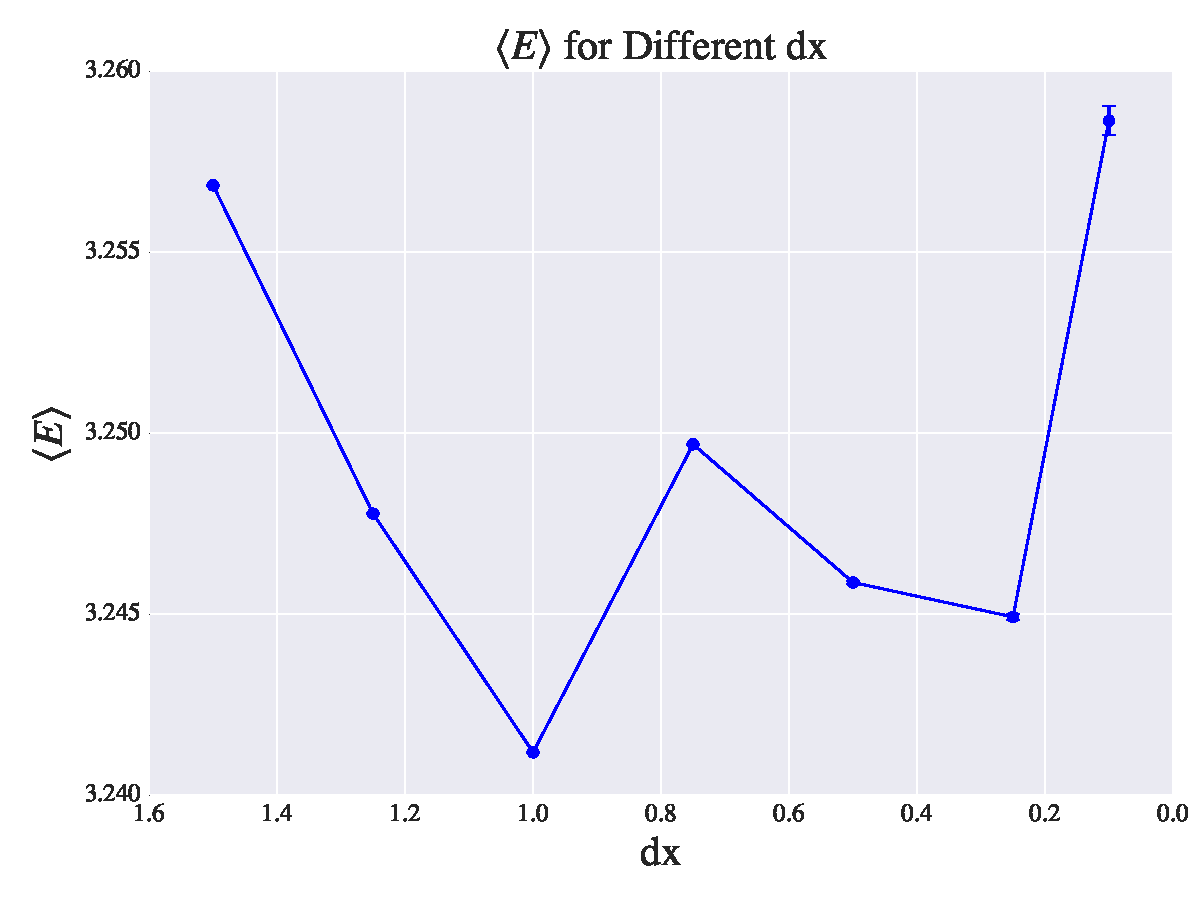
\includegraphics[width=\textwidth]{../Results/E_v_dx_normal_interacting.pdf}
	 		\caption{Mean of the energy}
	 	\end{subfigure}
	 	~
	 	\begin{subfigure}[b]{0.8\textwidth}
	 		\centering
	 		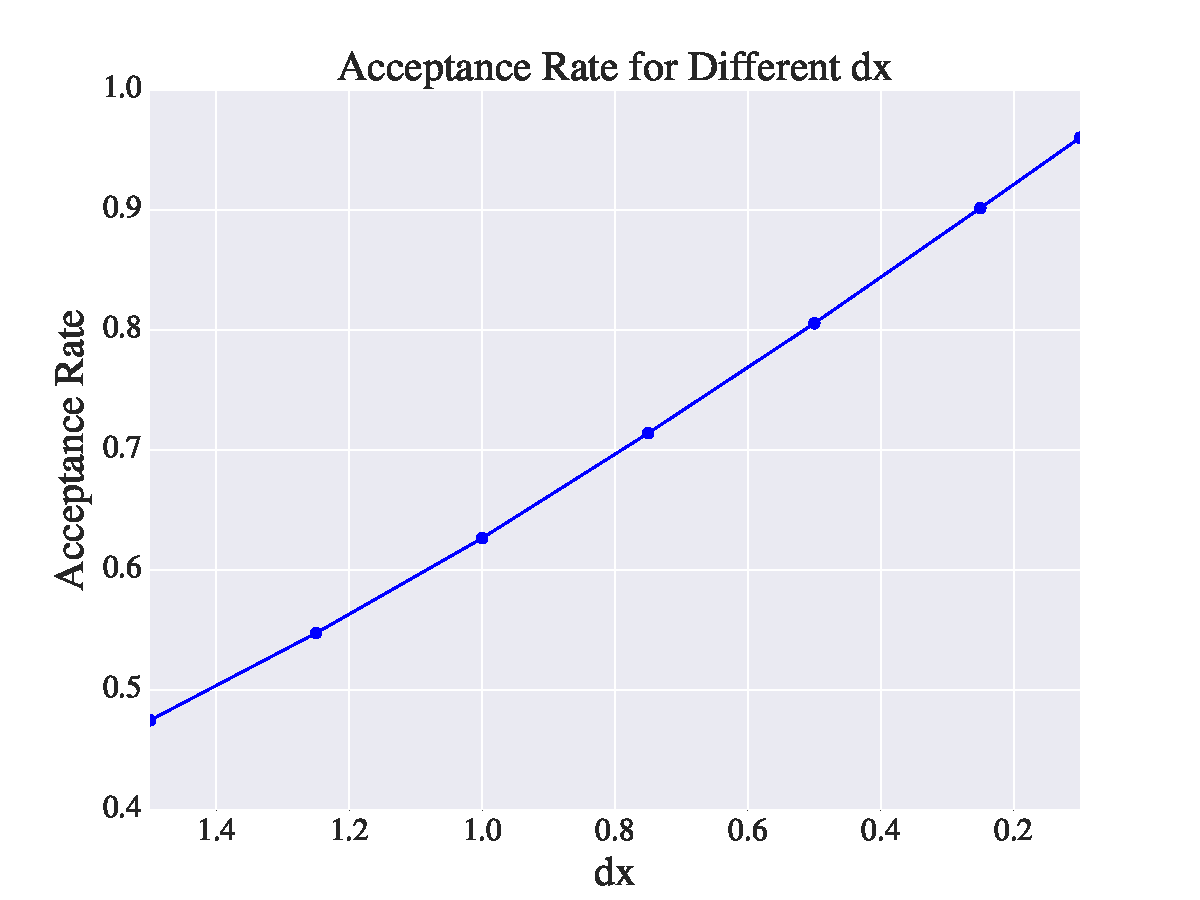
\includegraphics[width=\textwidth]{../Results/AC_normal_interacting.pdf}
	 		\caption{Acceptance ratio}
	 	\end{subfigure}
	 	\caption{Plot of the mean energy and corresponding acceptance rate for various values of $dx$ using $2$ particles in $2$ dimensions and $2^{20}$ Monte Carlo steps. This was produced using brute-force Metropolis sampling with $N=2, \gamma=0.3$ and $\sigma=1$}\label{fig:results_benchmark_no_importance_interacting}
	 \end{figure}
	 As explained in section \textbf{SECTION}, we choose $dx=1$ in this case. We show the equivalent plot with importance sampling in figure \ref{fig:results_benchmark_importance_interacting}
	 \begin{figure}[ht!]
	 	\centering
	 	\begin{subfigure}[b]{0.8\textwidth}
	 		\centering
	 		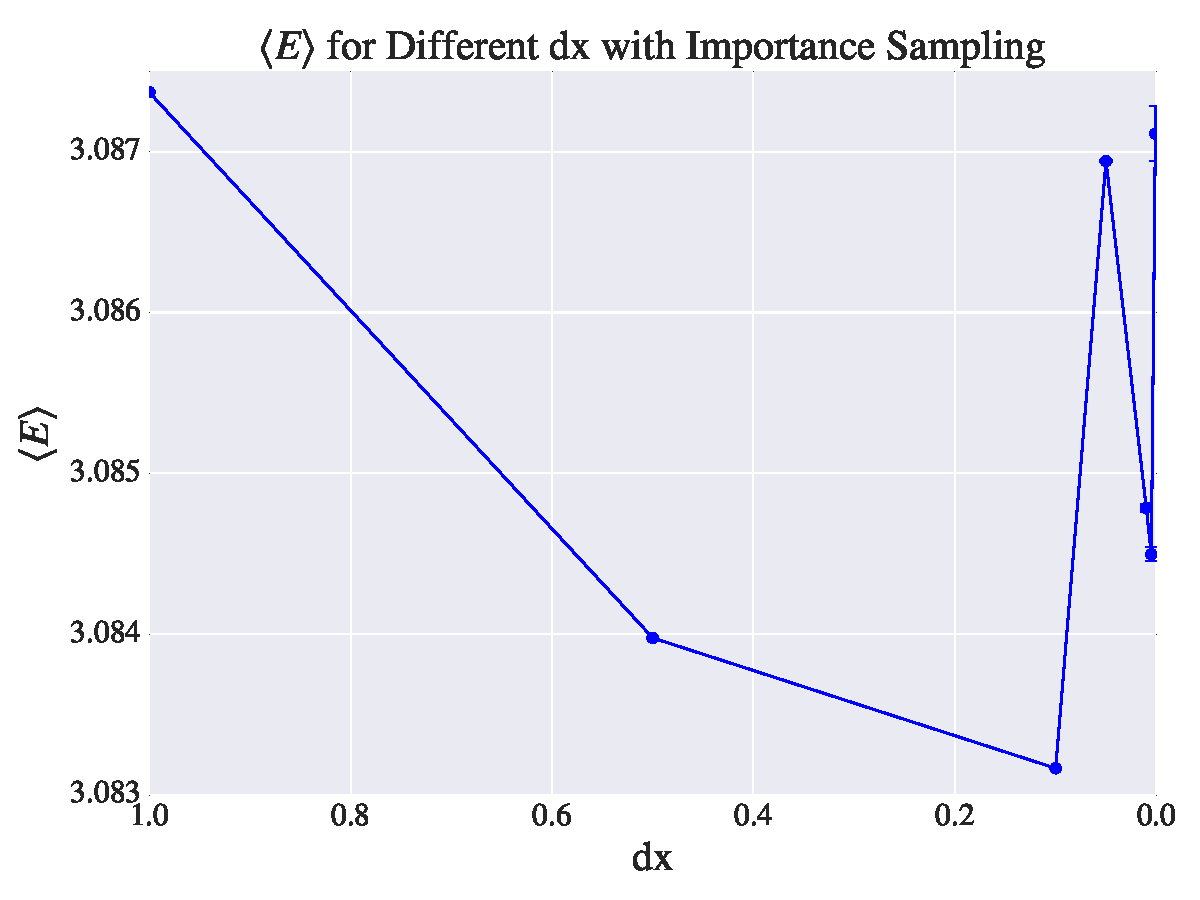
\includegraphics[width=\textwidth]{../Results/E_v_dx_importance_interacting.pdf}
	 		\caption{Mean of the energy}
	 	\end{subfigure}
	 	~
	 	\begin{subfigure}[b]{0.8\textwidth}
	 		\centering
	 		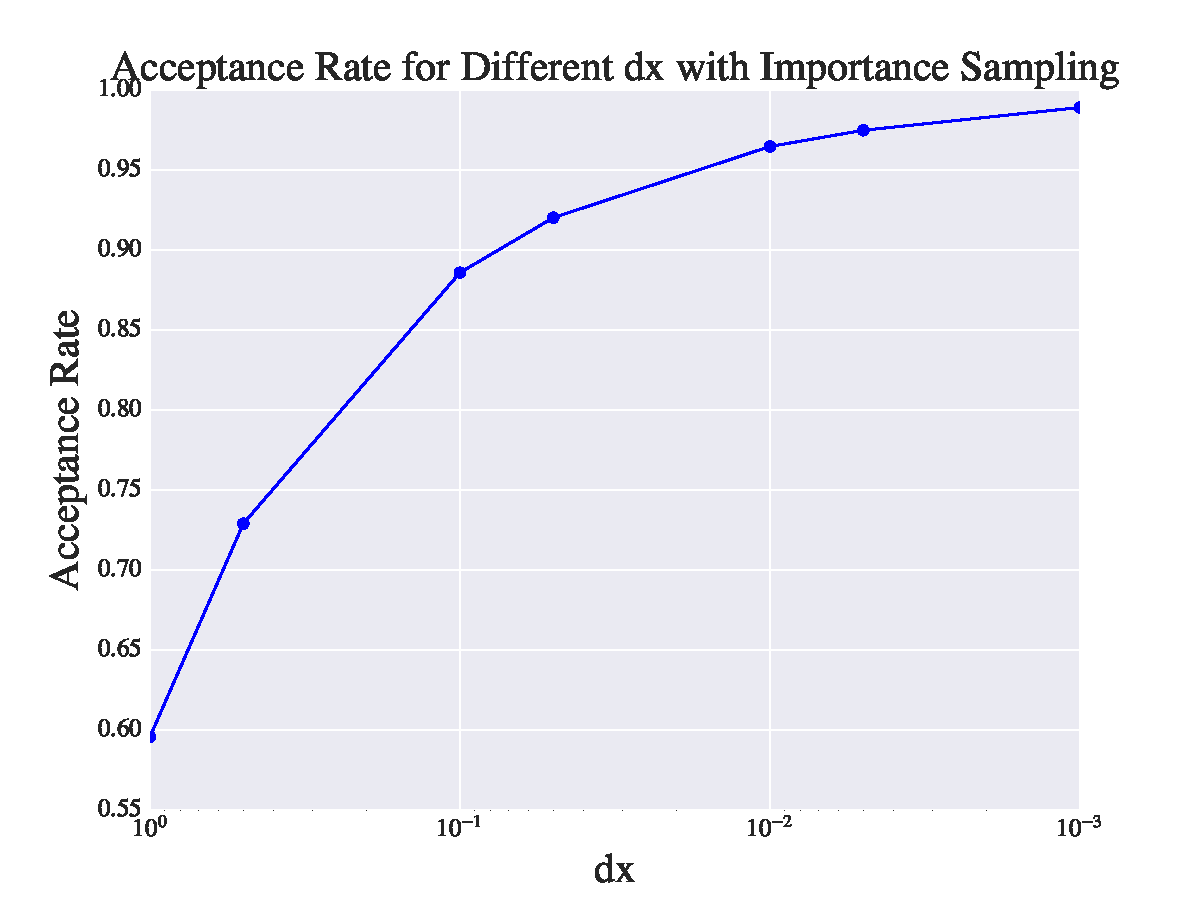
\includegraphics[width=\textwidth]{../Results/AC_importance_interacting.pdf}
	 		\caption{Acceptance ratio}
	 	\end{subfigure}
	 	\caption{Same as figure \ref{fig:results_benchmark_no_importance_interacting} but with importance sampling}\label{fig:results_benchmark_importance_interacting}
	 \end{figure}
	 As explained in section \textbf{SECTION}, we choose $dx=0.1$ in this case.
	 \subsubsection{Tuning $\boldsymbol{\sigma}$}
	As in the previous section, we also vary $\sigma$ in the interacting system, using Gibbs sampling. This is shown in figure \ref{fig:sigma_interacting}.
	 \begin{figure}
	 	\centering
	 	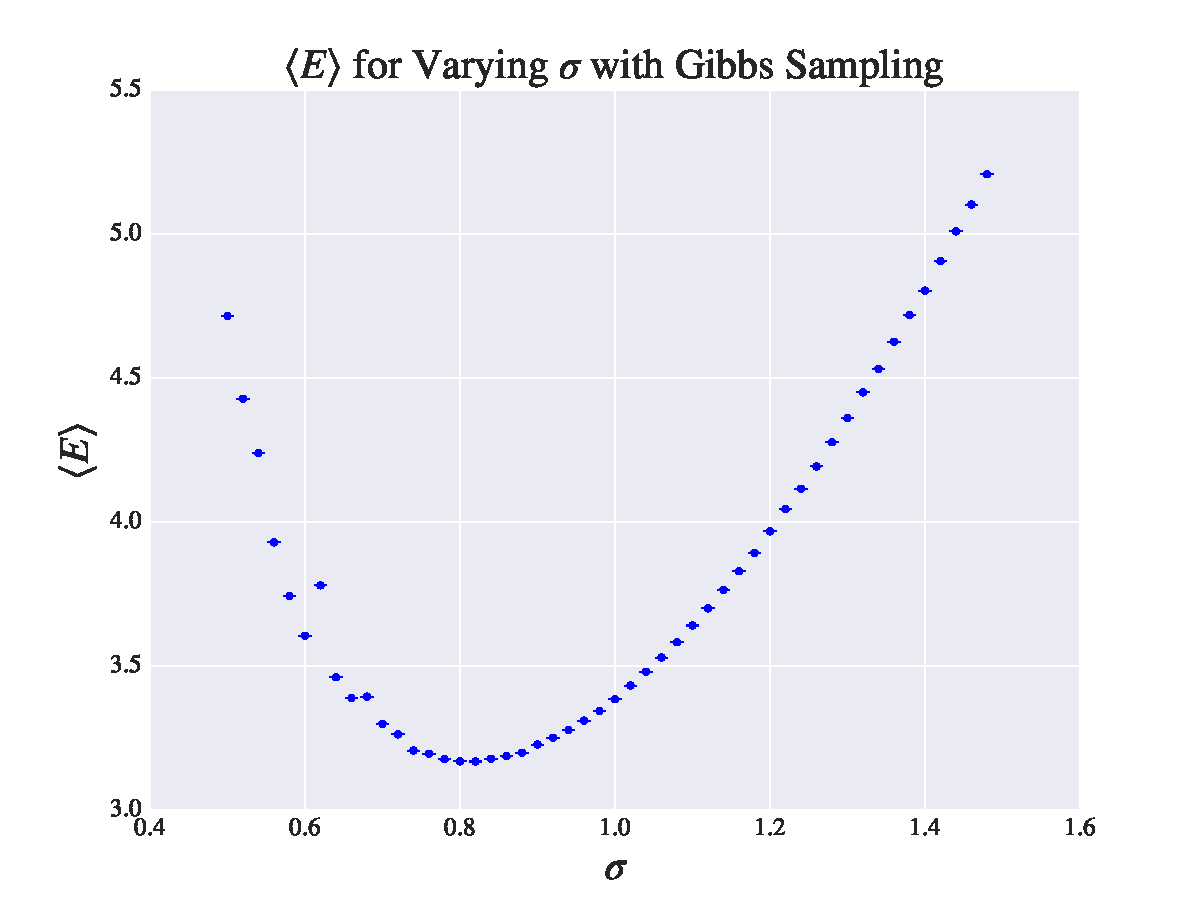
\includegraphics[width=\textwidth]{../Results/varying_sigma_gibbs_interacting.pdf}
	 	\caption{Mean energy as a function of $\sigma$ for an interacting system with $2$ electrons in $2$ dimensions, using $2^{20}$ Monte Carlo steps. This is with $N=2$ and $\gamma=0.05$ \textbf{CHECK THIS}}\label{fig:sigma_interacting}
	 \end{figure}
As explained in section \textbf{SECTION}, we choose $\sigma=0.82$ in this case.
	\section{Discussion}
	EXCELLENT DISCUSSION
	\section{Conclusion}
	BRILLIANT CONCLUSION
	\subsection{Outlook}
	MAGNIFICIENT OUTLOOK
	\bibliographystyle{apalike}
	\bibliography{Project2}
	\pagebreak
	\begin{appendices}
	\section{Finding the derivatives}\label{ap:finding_derivatives}
	In this section, we derive the expressions for the various derivatives needed in section \ref{sec:Theory}. We begin with the local energy.
	\subsection{The local energy}\label{ap:local_energy}
	The local energy is given by:
	\begin{equation}\label{eq:ap_local_energy}
	E_L=\frac{1}{\Psi_T}\hat{H}\Psi_T= \sum_{i=1}^N \left(-\frac{1}{2\Psi_T}\nabla_i^2 \Psi_T + \frac{1}{2}\omega^2 r_i^2\right)+\sum_{i<j} \frac{1}{r_{ij}}
	\end{equation}
	Thus, we must compute:
	\begin{equation}
	\frac{1}{\Psi_T}\nabla_i^2 \Psi_T
	\end{equation}
	This may be rewritten as:
	\begin{equation}\label{eq:log_expression_for_trial_wavefunction}
	\frac{1}{\Psi_T}\nabla \left(\Psi_T \frac{1}{\Psi_T} \nabla\Psi_T\right)=\left(\frac{1}{\Psi_T}\nabla \Psi_T\right)^2+\nabla \left(\frac{1}{\Psi_T}\nabla \Psi_T \right)=\left[\nabla \log \Psi_T\right]^2 + \nabla^2 \log \Psi_T
	\end{equation}
	The logarithm of our trial wavefunction is given by:
	\begin{equation}\label{eq:logarithm_of_wavefunction}
	\log \Psi_T = -\log Z -\sum_{i=1}^M \left(\frac{(X_i-a_i)^2}{2\sigma^2}\right)+\sum_{j=1}^N \log \left(1+\exp \left(b_j+\sum_{i=1}^{M} \frac{X_iw_{ij}}{\sigma^2}\right)\right)
	\end{equation}
	The derivative with respect to one coordinate is now given by:
	\begin{equation}\label{eq:first_derivative_log_psi}
	\begin{split}
	\frac{\partial \log \Psi_T}{\partial X_k}=\frac{(a_k-X_k)}{\sigma^2}+\sum_{j=1}^N \frac{w_{kj} \exp \left(b_j+\sum_{i=1}^{M} \frac{X_iw_{ij}}{\sigma^2}\right)}{\sigma^2 \left(1+\exp \left(b_j+\sum_{i=1}^{M} \frac{X_iw_{ij}}{\sigma^2}\right)\right)}\\
	=\frac{a_k-X_k}{\sigma^2}+\sum_{j=1}^N \frac{w_{kj}}{\sigma^2 \left(1+ \exp \left(-b_j-\sum_{i=1}^{M} \frac{X_iw_{ij}}{\sigma^2}\right)\right)}
	\end{split}
	\end{equation}
	Whereas the second derivative is:
	\begin{equation}\label{eq:second_derivative_log_psi}
	\frac{\partial^2 \log \Psi_T}{\partial X_k^2}=-\frac{1}{\sigma^2}+\sum_{j=1}^N \frac{w_{kj}^2 \exp \left(-b_j-\sum_{i=1}^{M}\frac{X_iw_{ij}}{\sigma^2} \right)}{\sigma^4\left(1+ \exp \left(-b_j-\sum_{i=1}^{M} \frac{X_iw_{ij}}{\sigma^2}\right)\right)^2}
	\end{equation}
	The local energy can now be found by using equation \ref{eq:log_expression_for_trial_wavefunction}, and inserting equation \ref{eq:first_derivative_log_psi} and equation \ref{eq:second_derivative_log_psi}. Inserting this into equation \ref{eq:ap_local_energy} gives the expression for the local energy stated in the main text.
	\subsection{The derivatives with respect to the parameters}\label{ap:derivative_parameters}
	For our optimization method, we require:
	\begin{equation}
	\frac{1}{\Psi_T}\frac{\partial \Psi_T}{\partial \alpha_k}=\frac{\partial }{\partial \alpha_k}\log \Psi_T
	\end{equation}
	Where $\alpha_k$ is any of the biases $a$, $b$ or the weights $w$ of the restricted Boltzmann machine. These derivatives are given by:
	\begin{equation}
	\frac{\partial \log \Psi_T }{\partial a_k}=\frac{X_k-a_k}{\sigma^2}
	\end{equation}
	\begin{equation}
	\frac{\partial \log \Psi_T}{\partial b_k}=\frac{\exp \left(b_k+\sum_{i=1}^M \frac{X_iw_{ik}}{\sigma^2}\right)}{1+\exp \left(b_k+\sum_{i=1}^M \frac{X_iw_{ik}}{\sigma^2}\right)}=\frac{1}{1+\exp \left(-b_k-\sum_{i=1}^M \frac{X_i w_{ik}}{\sigma^2}\right)}
	\end{equation}
	Finally, the derivative with respect to the coupling weights, $w_{kl}$ is given by:
	\begin{equation}
	\frac{\partial \log \Psi_T}{\partial w_{kl}}=\frac{X_k\exp\left(b_l+\sum_{i=1}^M \frac{X_iw_{il}}{\sigma^2}\right)}{\sigma^2\left(1+\exp \left( b_l + \sum_{i=1}^M \frac{X_iw_{il}}{\sigma^2}\right)\right)}=\frac{X_k}{\sigma^2\left(1+\exp \left(-b_l-\sum_{i=1}^M \frac{X_iw_{il}}{\sigma^2}\right)\right)}
	\end{equation}
	\subsection{The derivatives with Gibbs sampling}\label{ap:derivative_gibbs}
	In Gibbs sampling, we represent the wavefunction as $\Psi_{T, \mathrm{Gibbs}}=\sqrt{F_{rbm}(\boldsymbol{X})}$, instead of $\Psi_T=F_{rbm}(\boldsymbol{X})$. Note, however, that we only ever differentiate the logarithm of the wavefunction. As $\log \sqrt{\Psi_T}=\frac{1}{2}\log \Psi_T$, this gives only a marginal change. Specifically:
	\begin{equation}
	E_L=[\nabla \log \sqrt{\Psi_T}]^2 + \nabla^2 \log \sqrt{\Psi_T} =\frac{1}{4}[\nabla \log \Psi_T]^2 +\frac{1}{2}\nabla^2 \log \Psi_T
	\end{equation}
	\begin{equation}
	\frac{\partial }{\partial a_k}\log \sqrt{\Psi_T}=\frac{1}{2}\frac{\partial }{\partial a_k}\log \Psi_T
	\end{equation}
	\begin{equation}
	\frac{\partial }{\partial b_k}\log \sqrt{\Psi_T}=\frac{1}{2}\frac{\partial }{\partial b_k}\log \Psi_T
	\end{equation}
	\begin{equation}
	\frac{\partial}{\partial w_{kl}}\log \sqrt{\Psi_T}=\frac{1}{2}\frac{\partial}{\partial w_{kl}}\log \Psi_T
	\end{equation}
	Where the derivatives on the right-hand side are given in the previous section.
\section{Deriving the spin of the ground state wavefunction}\label{ap:Derivative_spin}
In this section we derive the spin of the exact two-particle ground state wavefunction in the noninteracting case.\\
\linebreak
Consider the unperturbed wavefunction for the ground state of the
two electron system, given by:
\begin{align}
\psi(\boldsymbol{r}_{1},\boldsymbol{r}_{2}) =
C\exp\left(-\omega\left(r_{1}^{2} + r_{2}^{2}\right)/2\right)
\end{align}
Since this wavefunction is symmetric under permutation of coordinate, the
Pauli exclusion principle states that the spin wavefunction must be antisymmetric function in to achieve a wavefunction that is totally antisymmetric under permutation of coordinates. This wave function must then be the singlet, and will look like:
\begin{align}
\ket{\psi} = \frac{1}{\sqrt{2}}\left(\ket{\uparrow} - \ket{\downarrow}\right)
\end{align}
This has spin $0$, as can be seen by applying the spin operator $\boldsymbol{S}^{2}$ to this state:
\begin{align}
\boldsymbol{S}^{2}\ket{\psi} = \frac{1}{\sqrt{2}}\left(
\underbrace{\boldsymbol{S}^{2}\ket{\uparrow}}_{= \frac{3}{4}\hbar^{2}} -
\underbrace{\boldsymbol{S}^{2}\ket{\downarrow}}_{= \frac{3}{4}\hbar^{2}}\right)
= 0
\end{align}
	\end{appendices}
\end{document}